%%%---PREAMBLE---%%%%%%%%%%%%%%%%%%%%%%%%%%%%
\documentclass[oneside,12pt,final]{sty/ucthesis-CA2012}
\pdfoutput=1

%--- Packages ---------------------------------------------------------
\usepackage[lofdepth,lotdepth,caption=false]{subfig}
\usepackage{fancyhdr}
\usepackage{hyperref}
\usepackage{amsmath, amssymb, graphicx}
\usepackage{xspace}
\usepackage{braket}
\usepackage{color}
\usepackage{setspace}
%\usepackage{subfigure} (Subfigure package clashes with another package)

%packags Laura added
\usepackage[utf8]{inputenc} %for the mac
\usepackage{multicol}
\usepackage[authoryear]{natbib}      %for bibliography parametrization (inline citations with square %brackets and author-year configuration)
\setcitestyle{round,aysep={},citesep={,}}    %round parenthesis, remove the comma between author and year, comma between citations https://gking.harvard.edu/files/natnotes2.pdf 
\let\cite\citep                             % make \cite command behave like \citep     
\usepackage{pdflscape}
\usepackage{lscape}
\usepackage{longtable}
\usepackage{booktabs}
\usepackage{float}


%---New Definitions and Commands------------------------------------------------------
\def\p{\partial}
\def\im{\mrm{im}}
\def\Tr{\mrm{Tr}}
\def\Z{\mbb{Z}}
\def\R{\mbb{R}}
\def\C{\mbb{C}}
\def\half{\frac{1}{2}}
\def\filler{\phantom{fillerfillerfiller}}
\newcommand{\be}{\begin{equation}}
\newcommand{\ee}{\end{equation}}
\newcommand{\mbb}[1]{\mathbb{#1}}
\newcommand{\mrm}[1]{\mathrm{#1}}
\newcommand{\mcal}[1]{\mathcal{#1}}
\newcommand{\mbf}[1]{\mathbf{#1}}
\newcommand{\ph}[1]{\phantom{#1}}
\newcommand{\udten}[3]{#1^{#2}_{\ph{#2}#3}}
\newcommand{\duten}[3]{#1^{\ph{#2}#3}_{#2}}
\newcommand{\pd}[2]{\frac{\p#1}{\p#2}}
\newcommand{\D}[2]{\frac{d#1}{d#2}}

%---Set Margins ------------------------------------------------------
\setlength\oddsidemargin{0.25 in} \setlength\evensidemargin{0.25 in} \setlength\textwidth{6.25 in} \setlength\textheight{8.50 in}
\setlength\footskip{0.25 in} \setlength\topmargin{0 in} \setlength\headheight{0.25 in} \setlength\headsep{0.25 in}

%%%---DOCUMENT---%%%%%%%%%%%%%%%%%%%%%%%%%%%%
\begin{document}

%=== Preliminary Pages ============================================
\begin{frontmatter}
	%%%%%%%%%%%%%%%%%%%%%%%%%%%
% TITLE PAGE INFORMATION %
%%%%%%%%%%%%%%%%%%%%%%%%%%%


\title{Uncertainty analysis in fisheries science--an interdisciplinary approach }

\author{Laura C. Urbisci}

%%%%%%%%%%%%%%%%%%%%%%%%%%%%%%%%%%
% DECLARATIONS FOR FRONT MATTER %
%%%%%%%%%%%%%%%%%%%%%%%%%%%%%%%%%%
\report{Dissertation} \degree{Doctor of Philosophy} \degreemonth{December} \degreeyear{2018}
\defensemonth{December} % should be one of the following: March, 
\defenseyear{2018}

\chair{Professor Steve Gaines}  % this is your advisor
\othermemberA{Professor Wendy Meiring} % This is a member of your committee 
\othermemberB{Doctor Kevin Piner} % This is a member of your committee 
\numberofmembers{3} % should match the number of entries above (chair + othermembers)

\field{Environmental Science \& Management}
\campus{Santa Barbara}


%\title{{ University of California \\ Santa Barbara} \linebreak \\  Ph.D. Dissertation}
%\author{Tom\'as Andrade}
%\date{2012}

	\maketitle
	\approvalpage
	\copyrightpage
	\begin{dedication}

\bigskip

${}$ \\

\bigskip

${}$ \\

\bigskip

${}$ \\

\bigskip

\begin{center}
\begin{Large}

I dedicate my dissertation to the countless cups of coffee, wine, and whiskey I consumed in the past 5.25 years. I could be nowhere with out you.

\end{Large}
\end{center}


\end{dedication} %comment out if you don't want a dedication
	\begin{acknowledgements}

There is a seemingly countless number of people I want to acknowledge who have supported me throughout my time in graduate school. 

\vspace{-\topsep}
\begin{itemize}
\setlength{\parskip}{0pt}
 \setlength{\itemsep}{0pt plus 1pt}
\item[--] Family: Thank you mummy and fasha for giving birth to me. You did a great job.
\item[--] PhD Committee: Thank you for all of your time, advice, and for putting up with all of my questions--both the smart and the dumb ones.
\item[--] Steve Gaines: You were my Thanksgiving toast. I'm so thankful for you.
\item[--] Hunter Lenihan: Even though our paths diverged, thank you for all of the lessons you taught me.
\item[--] My roommates: My roommates, my psuedo family, and my ``German friends". I love and thank you so much for everything you've done for me. House Dad (Spencer), House Child (Katrina), and House Goldfish (Mark), don't die without your House Mom. She's really going to miss you.
\item[--] Cubicle mate: Thank you Brian for all of the puns, for being an awesome study buddy through all of the PSTAT classes we took together, for being a patient sounding board to run ideas by, and for listening to me vent all my frustrations. Someday we'll win the lottery.
\item[--] Past and current lab mates: Thank you for all of your support the hugs and the listening. I'll always have chocolate for you.
\item[--] Bren buddies: Special shout out to Ian and Timbo. Thanks guys!
\item[--] Bren staff: Thank you Sage for all of your help my first year. Thank you Corlei, I know you no longer are at Bren, but you helped me so much when you were at Bren. You were the ultimate Bren Mom. Thank you Dee for being so helpful and a sweetheart. Thank you Kim for being the wonderful, unique you. Never change. Thank you Casey for being a friend in need. Thank you Kristine for being so supportive. Thank you Satie for guiding me along the way. Thank you Onella and Yoda. I loved getting to know you both. Thank you Doris for answering all of my emails. Sorry to bombard you all the time. Thank you Dave for all of your career advice. Thank you Geoff, Brad, and Steve for all of your computer help. Thank you Beth for joining me at all of our pro fem events. Fun times. Thank you Lisa for always taking the time to help me, no matter how busy you were. I really appreciate everything you've done for me.
\item[--] Bren faculty: Thank you Andrew Plantinga. I had a great experience working with you as a mentor on the MESM GP. Thank you Sarah Anderson for being super supportive. 
\item[--] PSTAT faculty: Thank you Prof. Jammalamadaka for being the professor of me dreams. I will always remember your catch phrase, ``Let's see what's cooking!" Thank you for Prof. Wang for being such a great teacher. I really enjoyed your lectures. Thank you Prof. Hsu. I still remember the time you thought I was doing my PhD in the PSTAT Department. I was so flattered. 
\item[--] PSTAT staff: Thank yooou Jamie. You're the best.
\item[--] NOAA/IATTC staff: Thank you Hoo Hoo and Carolina for always taking the time to help me.
\item[--]ERI staff: Thank you Erik Fields, St\'ephane Maritorena, and Dave Siegel for all of your help with SeaWiFS. 
\item[--] Ladies crew: Ladies, I love and appreciate you so much. I can't even put in words how much you mean to me. Timnit, Jessica, Phoebe, Julia, Lewam, and Alice. So much love going your way.
\item[--] Potluck and karaoke buddies: Mengya, Yuwei, Rungsheng, Ying, Yang, Jiajia, Zhitong, and Yuxiong--I've had such a great time hanging out with all of you. I've enjoyed all of our time together as friends. 
\item[--] Non-Bren grad school friends: Tara/Yuanbo, Zach, Ya, Anna, Sergio, and Ben--thank you for being such great friends and for all of the laughs.  Cool, cool.
\item[--] My mentors: Matt Burgess and Cody Szuwalski--I'm wishing the best for you in all of your endeavors.
\item[--] The Chalet Crew: Jen, Carl, Myley, Matt, Molly, Jacquie, Joe, and Mike--I've never been a group person, but you changed my mind
\item[--] Graduate Scholars family: my lovely mentoring family: Timnit, Terence, Natasha, and Xochitl and the GSP faculty and staff: Carlos, Michele, and Miros. I'm always here for you even if we are far apart.
\item[--] Other UCSB folks: Lana Hale-Smith and Megan Unden - I love you ladies. Thank you for being so helpful and validating.
\item[--] Thank you Deborah and Hap for being amazing role models and mentors.
\item[--] Funding sources: Dr. Daniel Vapnek Fellowship and Award, NMFS-Sea Grant Fellowship in Population and Ecosystem Dynamics (NOAA Grant $\#NA14OAR4170211$, California Sea Grant College Program Project $\#E/PD-13$), the Bren School, and the PSTAT Department.
\item[--] To all the dogs I ever dog sat--never forget me. And the owners too. Thanks for letting me get my doggo snuggles.
\end{itemize}
\vspace{-\topsep}

\end{acknowledgements} 
	\begin{vitae}
\addcontentsline{toc}{chapter}{Curriculum Vitae}

\begin{vitaesection}{\uppercase{Education}}
\vspace{-0.1cm}
\item [2018]	Ph.D. in Environmental Science \& Managemnt (Expected), University of California, Santa Barbara.
\item [2016]	M.A. in Applied Statistics, University of California, Santa Barbara.
\item [2012] 	BS in Environmental Science and Management \textit{with honors} Emphasis in Ecology, Biodiversity and Conservation, Minor in Spanish 
University of California, Davis 
\item  [2010] Education Abroad Program Universidad de Carlos III – Madrid, Spain
\end{vitaesection}

\textbf{\uppercase{Relevant Coursework}}
\begin{tabular}{l p{0.5\linewidth}}
Probability \& Statistics (3 part course) & Regression Analysis \\
Statistical Theory (2 part course) & Statistical Consulting \\
Advanced Statistical Methodology (3 part course) & Data Mining \\
Design and Analysis of Experiments & Time Series Analysis \\
Linear and Nonlinear Mixed Effects Modeling & Data Science \\
Bayesian Data Analysis & Machine Learning (audit) \\
\end{tabular}

\textbf{\uppercase{Relevant Statistical Experience}} \\
\textbf{Quantitative Consultant,} Santa Barbara, CA \\
\textit{Bren School of Environmental Science \& Management}
\hfill
9/16 – 3/17
\vspace{-\topsep}
\begin{itemize}
\setlength{\parskip}{0pt}
 \setlength{\itemsep}{0pt plus 1pt}
\item[--] Assisted all graduate students, faculty, postdocs, and visiting researchers with their quantitative needs 
\item[--] Advised the most appropriate statistical methods to use given the data set and research questions 
\item[--] Explained how to code statistical models and interpret model results
\end{itemize}
\vspace{-\topsep}

\textbf{Probability and Statistics Department,} UCSB	 \\
\textit{Group Projects}
\hfill				         
4/16 – 6/18
\vspace{-\topsep}
\begin{itemize}\setlength{\parskip}{0pt}
\setlength{\itemsep}{0pt plus 1pt}
\setlength\itemsep{0pt plus 1pt}
\item[--] Worked on a multiple projects that utilized different data sets including: biological and political
\item[--] Select skills applied include: principal component analysis, categorical KNN, classification tree analysis (with pruning, bagging, and random forests), and Naïve Bayes 
\item[--] Lead group by setting goals and determined course of action for a group of 4
\item[--] Presented ideas effectively and wrote a report which received positive feedback from instructor
\end{itemize}
\vspace{-\topsep}

\textbf{Probability and Statistics Department,} UCSB	 \\
\textit{Individual Projects}
\hfill
12/14 – 6/16
\vspace{-\topsep}
\begin{itemize}
\setlength{\parskip}{0pt}
\setlength{\itemsep}{0pt plus 1pt}
\item[--] Worked on a variety of projects to analyze results from various data sets including: medical, economic, and biological
\item[--] Overview of skills and select a few used: fitted a time series model (Seasonal ARIMA) to data and forecasted into the future to predict values, compared the efficacy of three weight-loss programs using linear mixed effects models, looked at the economic relationship between the 48 contiguous states using multivariate analysis methods and linear models
\item[--] Presented ideas effectively in project interview and wrote a report which received positive feedback 
\end{itemize}
\vspace{-\topsep}
 
\textbf{\uppercase{STATISTICAL LEADERSHIP EXPERIENCE}} \\
\textbf{Teaching Assistant (TA),} Santa Barbara, CA \\
\textit{University of California, Santa Barbara}
\hfill
3/17 – current
\vspace{-\topsep}
\begin{itemize}
\setlength{\parskip}{0pt}
\setlength{\itemsep}{0pt plus 1pt}
\item[--] Gave multiple guest lectures to ~ 150 students on linear regression, binomial proportion test, and chi-squared tests
\item[--] Managed computer labs and showed students how to program in R, the R GUI R Commander, SAS, and Excel
\item[--] Taught material ranging from basic statistical concepts to advanced statistical theory to students who came from a wide range of backgrounds
\end{itemize}
\vspace{-\topsep}

\textbf{Statistics Tutor,} Santa Barbara, CA \\
\textit{Probability and Statistics Department}		
\hfill
9/15 – current
\vspace{-\topsep}
\begin{itemize}
\setlength{\parskip}{0pt}
\setlength{\itemsep}{0pt plus 1pt}
\item[--] Aided undergraduate students with their quantitative coursework and taught R
\item[--] Helped students understand difficult concepts by explaining it to them in novel ways
\end{itemize}
\vspace{-\topsep}

\textbf{Master’s Group Project PhD Mentor,} Santa Barbara, CA \\
\textit{Bren School of Environmental Science \& Management}
\hfill
3/16 – 3/17
\vspace{-\topsep}
\begin{itemize}
\setlength{\parskip}{0pt}
\setlength{\itemsep}{0pt plus 1pt}
\item[--] Helped master student’s set attainable goals, define research questions, and develop a feasible project timeline
\item[--] Reviewed and provided feedback on drafts of reports and presentations
\item[--] Recommended appropriate statistical analysis given data
\end{itemize}
\vspace{-\topsep}

\textbf{Intern,} La Jolla, CA \\
\textit{NOAA Southwest Fisheries Science Center}		
\hfill
8/12 – 8/13
\vspace{-\topsep}
\begin{itemize}
\setlength{\parskip}{0pt}
\setlength{\itemsep}{0pt plus 1pt}
\item[--] Analyzed scientific data and presented findings at a professional meeting
\item[--] Trained lab assistants 
\end{itemize}
\vspace{-\topsep}
 
\textbf{\uppercase{Publications}} \\
\textbf{Urbisci, L. C.}, Stohs, S. M., and Piner, K. P. 2017. From sunrise to sunset in the California drift gillnet fishery: An examination of the effects of time and area closures on the catch and catch rates of four key pelagic species: thresher shark (Alopias vulpinus), swordfish (Xiphias gladius), blue shark (Prionace glauca), and shortfin mako (Isurus oxyrinchus). Marine Fisheries Review. 78(3-4):1-12. 

Ayres, A., Degolia, A., Fienup M., Kim J., Sainz, J., \textbf{Urbisci, L. C.}, Viana, D., Wesolowski, G., Plantinga, A. J., Tague, C. 2016. Social science/natural science perspectives on wildfire and climate change. Geography Compass. 10.2: 67-86.

\textbf{Urbisci, L. C.}, Sippel, T., Teo, L. H., Piner, K. R., and Kohin, S. 2013 Size composition and spatial distribution of shortfin mako sharks by size and sex in U.S. West Coast fisheries. Submitted to ISC Shark Working Group Workshop July 6-11, 2013. 

\textbf{Urbisci, L. C.,} Runcie, R., Sippel, T., Piner, K., Dewar, H., and Kohin, S. 2012 Examining size-sex segregation among blue sharks (Prionace glauca) from the Eastern Pacific Ocean using drift gillnet fishery and satellite tagging data.  Submitted to ISC Shark Working Group Workshop January 7-14, 2013. 

\textbf{Urbisci, L. C.} 2011. Testing the unknown: the distribution, size and abundance of intertidal Haliotis rufescens (red abalone) and Haliotis cracherodii (black abalone) within Marine Protected Areas. (Unpublished student report. On file at the Cadet Hand Library, U.C. Davis Bodega Marine Laboratory). 


\textbf{\uppercase{Presentations}} \\
\textbf{Urbisci, L.C.} 2018. Untangling uncertainty in food webs. Presented to Schmidt Family Foundation on March 9, 2018, Santa Barbara, CA. 

\textbf{Urbisci, L.C.} 2017. Fishing through the food web leads to systematic overestimation of maximum sustainable yield. Presented at the NMFS-SG Annual Fellows Meeting on May 8-10, 2017, Beaufort, NC. 

\textbf{Urbisci, L.C.}, 2016. Developing an alternative estimate for virgin biomass using food web dynamics. Presented at the NMFS-SG Annual Fellows Meeting on June 28-30, 2016, Santa Cruz, CA.

\textbf{Urbisci, L.C.}, 2016. Developing an alternative estimate for virgin biomass using food web dynamics. Presented at the Bren School PhD Symposium on February 19, 2016, Santa Barbara, CA.

\textbf{Urbisci, L.C.}, 2015. Developing a new ecosystem‐based management approach: using ecosystem model to calculate a better estimate of population scale for single‐species models. Presented at the NMFS-SG Annual Fellows Meeting on June 9-11, 2015, Miami, FL.

\textbf{Urbisci, L.C.}, Stohs, S. M., and Piner, K. P. 2014. From sunrise to sunset in the California drift gillnet fishery: An examination of the effects of time and area closures on the catch and catch rates of four key pelagic species: thresher shark (Alopias vulpinus), swordfish (Xiphias gladius), blue shark (Prionace glauca), and shortfin mako (Isurus oxyrinchus). Presented at the Highly Migratory Species Management Team Meeting on January 22, 2014, La Jolla, CA.

\textbf{Urbisci, L.C.} Runcie, R., Sippel, T., Piner, K., Dewar, H., and Kohin, S. 2012 Examining size-sex segregation among blue sharks (Prionace glauca) from the Eastern Pacific Ocean using drift gillnet fishery and satellite tagging data.  Presented at the ISC Shark Working Group Workshop January 10, 2013. 

\textbf{Urbisci, L.C.} 2011. Testing the unknown: the distribution, size and abundance of intertidal Haliotis rufescens (red abalone) and Haliotis cracherodii (black abalone) within Marine Protected Areas. Presented at the Sequence One and Two Student Symposium 2011, Bodega Bay, CA.

\end{vitae}
	%
%  Abstract
%

\begin{abstract}
\addcontentsline{toc}{chapter}{Abstract}
%todo: max 350 words

Laura's dissertation is an interdisciplinary approach that combines fisheries science, ecological theory, and applied statistics. Her first chapter is a meta-analysis on transfer efficiency that describes and quantifies the variation in transfer efficiency. Her second chapter assesses uncertainty in food web models by creating multiple Monte Carlo simulations to test various ecological assumptions about net primary production and transfer efficiency. Her final chapter is a comparative analysis of two Bayesian models: a classic Bayesian surplus production model and a Bayesian surplus production model that incorporates ecological information. This chapter examines if the inclusion of ecological information informs and alters fisheries assessment models, with a focus on data-limited fisheries. Ultimately, Laura's work bridges the gap between applied statistics and ecological theory and encourages the use of uncertainty analysis to make more robust predictions in food web models.

%\abstractsignature
\end{abstract}



	\tableofcontents
\end{frontmatter}

\begin{mainmatter}

%---Set Headers and Footers ------------------------------------------------------
\pagestyle{fancy}
\renewcommand{\chaptermark}[1]{\markboth{{\sf #1 \hspace*{\fill} Chapter~\thechapter}}{} }
\renewcommand{\sectionmark}[1]{\markright{ {\sf Section~\thesection \hspace*{\fill} #1 }}}
\fancyhf{}

\makeatletter \if@twoside \fancyhead[LO]{\small \rightmark} \fancyhead[RE]{\small\leftmark} \else \fancyhead[LO]{\small\leftmark}
\fancyhead[RE]{\small\rightmark} \fi

\def\cleardoublepage{\clearpage\if@openright \ifodd\c@page\else
  \hbox{}
  \vspace*{\fill}
  \begin{center}
    This page intentionally left blank
  \end{center}
  \vspace{\fill}
  \thispagestyle{plain}
  \newpage
  \fi \fi}
\makeatother
\fancyfoot[c]{\textrm{\textup{\thepage}}} % page number
\fancyfoot[C]{\thepage}
\renewcommand{\headrulewidth}{0.4pt}

\fancypagestyle{plain} { \fancyhf{} \fancyfoot[C]{\thepage}
\renewcommand{\headrulewidth}{0pt}
\renewcommand{\footrulewidth}{0pt}}

%=== Introduction ============================================
\chapter{Introduction}
Fisheries modeling take the complexity of a single heterogeneous stock with different sizes, ages, growth rates, movement patterns, reproductive abilities, behaviors in response to fishing gear, and risks of natural mortality and simplify these diverse dynamics into a cohesive model. These stock assessment models look at data such as the number of fish caught, total biomass over a certain range, catch per unit area, and mean size (weight or length) of fish harvested and attempt to predict how these attributes will respond to fishing over time. Depending on the available data and level of complexity desired, we can model open ocean ecosystems using several different approaches. Most models focus on an individual stock and fall under the category of a single-species model. The simplest single-species models look only at abundance and are referred to as biomass dynamic or production models. These models can be extended in three ways. They can include age-structure, the dynamics of fleets, spatial structure, and interactions with other species and the environment. The models that include species interactions and environmental fluctuations are a special class of models referred to as ecosystem-based models.

\vspace{5mm}

A multitude of ecosystem-based models have been developed within the past three decades to address the need to incorporate ecosystem-based science into fisheries management. These models help inform decision-makers about the effects of fishing mortality and the indirect trophic implications of fishing in changing ecological environments. There are various types of ecosystem-based models: whole ecosystem and dynamic system models, minimum realistic models (restrict a model to those species most likely to have important interactions with the species of interest), individual-based models (follow an individual through their life cycle), and bioenergetics models (use bioenergetics and allometric reasoning) \cite{plaganyi2004critical,collie2014ecosystem}. All of these classes of models aim to simulate the environment by including species interactions and environmental fluctuations. 

\vspace{5mm}

Instead of attempting to explain all the ecological processes in one model, a new possible approach is to move away from focusing on small-scale details and look at the ecosystem in a broader context. We can combine ecosystem-knowledge to improve upon single-species models. For instance by applying ecological theory such as food web dynamics, we can develop a more feasible approach to estimate the unfished biomass and carrying capacity. By taking the amount of net primary production that enters into the system, we can use the principle behind energy transfer in food webs to approximate the amount of biomass at each trophic level. By taking a bottom-up approach, we can ensure that our estimates of unfished biomass are feasible, because we account for how much energy goes into the system. We can additionally include sensitivity analysis in our model to account for the natural variation in the environment.

%\begin{section}{Permissions and Attributions}
%\begin{enumerate}
%
%\item The content of chapter 2 and appendix A is the result of a collaboration with Alice and Bob, and has previously appeared in the (Journal) (paper citation). It is reproduced here with the permission of (Institution): \url{http://}.
%
%\end{enumerate}
%\end{section}

%=== Chapter 1 ============================================
\chapter{Tangled is the web we weave}
%---  Section -------------------------
\section{Introduction}
One of the crucial, and at times, most puzzling concepts in food web dynamics research is the transfer efficiency-?the movement of production between trophic levels. This paper addresses two aspects of transfer efficiency: first, we seek to provide clarity and untangle the web of confusion surrounding the conceptualization of transfer efficiency. Second, we address the often-cited claim that transfer efficiency is a constant 10\%. We analyze extant research to show that transfer efficiency varies substantially across systems, trophic levels, and taxa. 

\subsection{Origin and conceptualization of transfer efficiency}
The definition of transfer efficiency has been somewhat muddled since its inception. We refer to transfer efficiency as the fraction of production passing from one trophic level to the next \cite{slobodkin1959energetics}. At times it has also been referred to as trophic (transfer) efficiency \cite{chapman1998ecology}. This term is often confused with other non-equivalent efficiencies such as ecological efficiency, assimilation efficiency, and consumption efficiency \cite{iverson1990control, hairston1993causeeffect}. However, each of these efficiencies addresses distinct ecological questions and thus require different data for their calculations. \citet{slobodkin1959energetics} theorized a food chain efficiency metric and defined it as the ratio of the number of organisms removed from the targeted population to the food consumed by the targeted population \cite{slobodkin1960ecological,slobodkin1962energy}. Removal includes both natural mortality and human harvesting. He subsequently renamed the concept ``ecological efficiency" in his 1962 and 1972 papers \cite{slobodkin1962energy, slobodkin1972inconstancy}. The energy budget requires a balance between inputs and outputs. When energy is ingested, some of that energy is lost to respiration and excretion. Then, the remaining energy that is assimilated is divided amongst basal maintenance, growth, and reproduction. Assimilation efficiency is defined as the percentage of energy ingested at trophic level $n$ that is assimilated at trophic level $n$ \cite{hairston1993causeeffect}. The consumption efficiency measures the number of organisms from the prey population that is consumed by its predators and is defined as the percentage of net production at trophic level $n$ that is consumed by trophic level $n + 1$ \cite{hairston1993causeeffect}. In an attempt to make the differences clearer, we provide a simple cartoon of a food web (Figure \ref{foodweb}) that visualizes the definitions of four of the commonly used efficiencies. 

\vspace{5mm}

Availability of data differs between ecosystems. It is difficult in aquatic systems, especially marine systems, to gather enough data on every species in order to calculate the assimilation and consumption efficiencies. Terrestrial studies, on the other hand, can collect detailed population data much easier. Thus, terrestrial studies do not need to rely as much on inferential techniques, like the transfer efficiency, and have the ability to calculate species-specific metrics, such as the assimilation and consumption efficiency. To clarify, the assimilation and consumption efficiencies can also be calculated at the trophic-level in addition to the species-level.

\begin{figure}[H]
     \centering
       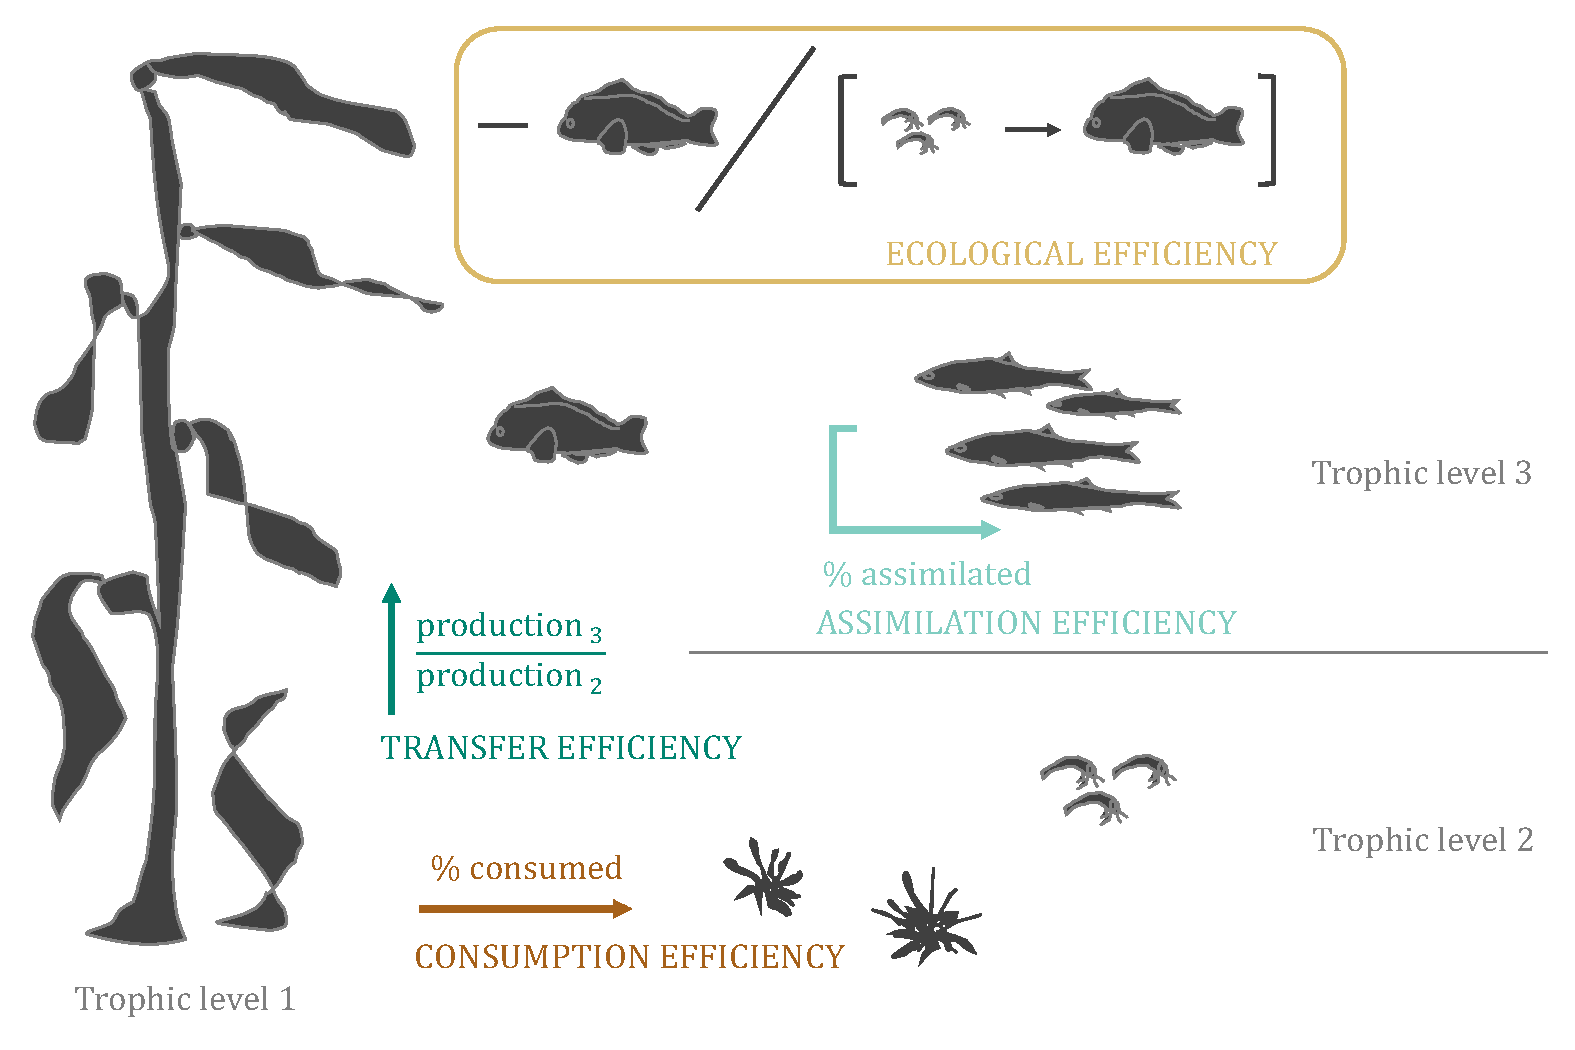
\includegraphics[width=\textwidth]{fig/foodwebimage}
    \caption{Cartoon of a food web that visualizes different efficiencies. The consumption efficiency is in brown, the transfer efficiency is in teal, the assimilation efficiency is in light blue, and the ecological efficiency (food chain efficiency) is in tan. In the consumption and ecological efficiency, the head of the arrow indicates the direction of consumption, where the species at the arrow head represent the species consuming the species at the arrow's origin. The diagram of the ecological efficiency includes a negative sign, division sign, and parentheses. Plot created using Microsoft office 2013.}
    \label{foodweb}
\end{figure}

The confusion around the definition is not the only complication with transfer efficiency--the values themselves have been disputed over the years and remain a point of contention. It is surprising that some scholars treat transfer efficiency as a fixed constant (i.e., 10\%) for all trophic levels in light of the fact that other scholars have found that physiological, and potentially behavioral, characteristics influence transfer efficiency \cite{may1983ecology, pauly1995primary, ware2000aquatic, cury2005trophodynamic, libralato2008novel, chassot2010global, trebilco2013ecosystem, watson2014primary}.

\subsection*{Physiological and behavioral characteristics of transfer efficiency in freshwater and marine ecosystems}
Multiple factors have been shown to affect transfer efficiency in both freshwater and marine ecosystems. In freshwater systems, the sources of variability in transfer efficiencies include the body of water, season, trophic level, and species composition \cite{lindeman1942trophic, gaedke1994seasonal, rybarczyk2003analysis, karlsson2007differences}.
In marine systems, transfer efficiency varies by ecological system, geographic location, trophic level, metabolic strategy, and species composition \cite{may1983ecology, persson2007food, libralato2008novel, barnes2010global}.

\subsubsection*{Ecological system within freshwater and marine ecosystems}
Transfer efficiency has been found to be specific to the geographical region. Multiple marine studies found distinct transfer efficiencies between upwelling, temperate and tropical ecosystems (i.e., 5\% upwelling, 10\% temperate, and 14\% tropical) \cite{libralato2008novel, coll2008ecosystem, chassot2010global}. Even within a single ecosystem,
\citet{baird2004energy} found that each community within an intertidal ecosystem had unique transfer efficiency values. Distinct transfer efficiency values have also been found to occur not only between lakes and within trophic levels in freshwater ecosystems \cite{lindeman1942trophic}, but also in bays and estuaries as well \cite{rybarczyk2003analysis}.

\vspace{5mm}

Additionally, research has found that the amount of sunlight a region receives affects transfer efficiency. \citet{sanmartin2006latitudinal} suggest that transfer efficiency from phytoplankton to zooplankton in marine ecosystems decreases as latitude increases due to the decrease in sunlight. \citet{gaedke1994seasonal} found seasonal variation in transfer efficiency between the first and second trophic level in lakes, with transfer efficiency rising in the summer and fall and decreasing in the winter and spring. The seasonal variation in transfer efficiency can be attributed to the decrease in phytoplankton abundance in winter due to limited sunlight. As daylight increases in early spring, there is a gradual increase in phytoplankton blooms--culminating in the maximum phytoplankton production in summer (i.e., peak hours of sunlight).  As the days become shorter in fall and the hours of sunlight decreases, there is a decrease in the amount of phytoplankton. There is a time lag corresponding to the change in sunlight in the spring and fall seasons. Therefore, the amount of sunlight indirectly influences transfer efficiency between the first and second trophic level by directly impacting the phytoplankton abundance. 

\subsubsection*{Trophic level}
Size spectrum studies report that transfer efficiency decreases with body size, and by association, trophic level \cite{barnes2010global}. Therefore, the size ratio of prey to predators (e.g., phytoplankton to zooplankton) impacts transfer efficiency and trophic structure 
\cite{havens1998size, garciacomas2016prey}.

\subsubsection*{Metabolic strategy}
Furthermore, \citet{may1983ecology} found ectotherms are more efficient than endotherms in transferring energy from trophic level $n$ to trophic level $n+1$, with energy transfer efficiencies around 20-50\% for invertebrate ectotherms, around 10\% for vertebrate ectotherms and less than 2\% for endotherms. This discrepancy in transfer efficiency is due to the metabolic efficiency: ectotherms rely on environmental heat sources and therefore have a lower metabolic cost in comparison to endotherms. Much of the metabolic energy in endotherms goes to the production of heat. Therefore, transfer of energy in the higher trophic levels where endotherms are prominent is less than the lower trophic levels were ectotherms make up more of the composition in marine ecosystems \cite{mcgarvey2018two}.

\subsubsection*{Species composition}
Consuming nutritionally imbalanced food has been shown to lead to large respiratory losses, which negatively affect transfer efficiency \cite{persson2007food}. \citet{karlsson2007differences} and \citet{vonelert2003absence} found that the species composition of prey, in particular different species of zooplankton crustaceans and the absence of long-chain polyunsaturated fatty acid in cyanobacteria, influence transfer efficiency. In addition, the presence of jellyfish blooms has been found to reduce the transfer of energy to higher trophic levels \cite{condon2011jellyfish}.

\vspace{5mm}

\citet{trussell2006fear} and \citet{schmitz2008individuals} found that the risk of predation modifies prey conversion efficiencies and biomass production, which could therefore influence trophic structure and energy transfer. While these results refer specifically to assimilation and consumption efficiencies, it is plausible that this behavior influences transfer efficiencies as well. While the specific factors  previously discussed influence transfer efficiency individually, these components interact in the natural environment. Because of this interaction, researchers must consider the impacts of the synergistic effects of these factors on the variability of the transfer efficiency and in turn how to account for them in the modeling process.  

\subsection*{The 10\% transfer efficiency}
Although the studies above highlight that a number of factors can greatly affect trophic efficiencies, we still see broad use of the assumption of a constant value of 10\%. To explore how (un)reasonable this assumption might be in different contexts, we synthesize the pattern of variation that has been observed in empirical studies that measured transfer efficiencies. Our goal is to provide guidance for what is reasonable to assume and what is necessary to measure.

\vspace{5mm}

It is unclear where the 10\% transfer efficiency assumption came from. Looking back at the historical records, we find a ``tangled web" of misattributions and a general lack of empirical evidence. \citet{semper1881animal} might have come up with the theory that there is a 10\% transfer between trophic levels, but he lacked empirical evidence to back this claim \cite{mcintosh1986background}. \citet{lindeman1942trophic} developed more general theory by looking at energy flow diagrams and mentioned a progressive efficiency which is currently known as transfer efficiency. However, no explicit mention of a 10\% value shows up in this work even though he is often credited for it (i.e., Lindeman?s law of trophic transfer efficiency--\citealt{chapman1998ecology}). \citet{slobodkin1959energetics, slobodkin1972inconstancy} stated that ?the values mentioned by Lindeman, as well as other values presented by other field workers, for ecological efficiency tended to cluster around 10\%.? Yet, Lindeman never explicitly discusses the ecological efficiency. He talked about the progressive efficiency, which as mentioned previously is a different concept. Regardless, Slobodkin and his students used laboratory experiments to formalize the hypothesis that there was an approximately 10\% transfer between trophic levels \cite{slobodkin1959energetics}. He referred to this as the food chain efficiency, which was later renamed to the ecological efficiency. However in a later study, \citet{slobodkin1972inconstancy} found empirical and theoretical objections to the 10\% ecological efficiency and rejected the theory. According to \citet{mcintosh1986background}, ?Nevertheless, May (1967b) in pursuit of the ?perfect crystals? of ecology, included Slobodkin?s 1961 hypothesis in a series of community properties he described as ?constant and predictable?.? In a more recent edition of May?s Theoretical Ecology textbook , however, the authors reach a very different conclusion:

\begin{quote}
One such [generalization] in the early 1960s suggested that the food-chain efficiency for transfer of energy from one trophic level to the next was generally around 10\%. Subsequent studies showed that such food-chain efficiencies can vary over two or more orders of magnitude, from less than 0.1\% to significantly more than 10\%. Some evidence suggests such efficiencies may, other things being equal, be higher for carnivores and detritus feeders than for herbivores, possibly because biochemical conversion efficiencies are higher for animals eating plants. \cite{may2007theoretical}
\end{quote}

In Figure \ref{flowchart}, we present a flowchart showing the muddled origin of this concept. Given the unclear origin and application of the 10\% transfer efficiency assumption, this assumption warrants further analysis, which is the focus of this current study. In the following section, we synthesize studies that provide empirical estimates of transfer efficiencies.

\begin{figure}[H]
     \centering
       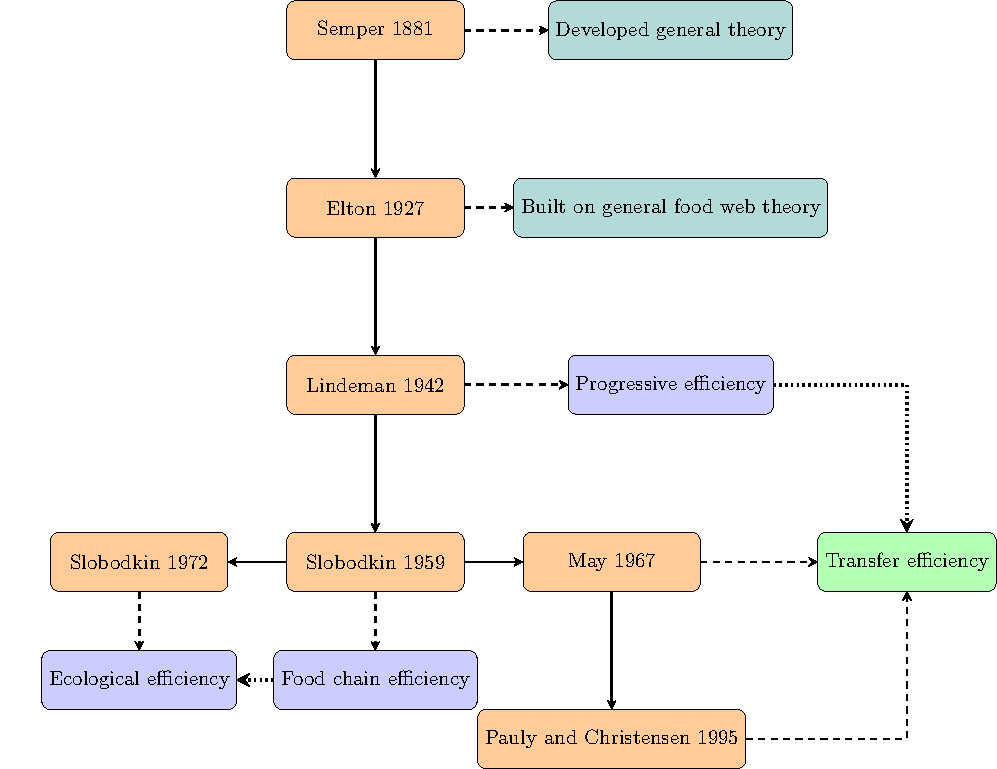
\includegraphics[width=\textwidth]{fig/flowchartfig}
    \caption{Flow chart of the origin of the 10\% transfer efficiency theory (green icon). A subset of key journal articles are highlighted in the orange icons. The dashed lines point to the efficiency mention in a particular article. The dotted lines represent a change in the name of an efficiency. Teal icons denote that the article discussed general theory, while periwinkle blue icons represent the discussion of a type of efficiency. The arrowhead attached to the solid line denotes the downstream flow direction of citations. Plot created using LaTeX v.2.9.6211  \cite{lamport1994latex} package tikz v.3.0.1a \cite{tantau2015tikz}.}
    \label{flowchart}
\end{figure}

\section*{Methods}
To explore the empirical distributions of transfer efficiencies, we collected  articles that mentioned both food web and transfer efficiency. We then selected from these studies those that included relevant data, whether model-based or empirical. While we initially hoped to include terrestrial as well as freshwater and marine studies, we found nearly all of the terrestrial studies were on the consumption and assimilation efficiency, not the transfer efficiency. Therefore, we broke our analysis into two sections: freshwater and marine and ignored terrestrial. We primarily applied exploratory data analysis techniques such as summary statistics to distinguish patterns between the systems. 

\vspace{5mm}

If the sample size was sufficient large, we also used decision tree analysis (i.e., regression trees with pruning, bagging, and random forests) and Monte Carlo simulations (See Table \ref{datafresh} and \ref{datamar}). Decision tree analysis was employed to determine which factors had the largest impact on transfer efficiency. Using an approach similar to \cite{libralato2008novel}, we clustered the marine ecosystems into the following regions: temperate shelves and seas, tropical shelves and seas, lagoons, upwelling ecosystems, and open oceans. Although we also clustered the freshwater ecosystems into lakes, springs, and ponds, the sample size of the freshwater transfer efficiency data was too small to run regression tree analysis. We used regression trees with pruning, bagging, and random forests on the marine transfer efficiency data set and used relative importance plots to determine which factors accounted for the largest sources of variation and were most useful in predicting transfer efficiency. In the discussion, we used Monte Carlo simulations to aid in the conversation.

\subsection*{Freshwater}
Many of the preliminary studies on transfer efficiency occurred in freshwater systems. All of the early studies were empirical (i.e., data used to calculate the transfer efficiency were collected either through laboratory experiments or from the field), but over time studies shifted to being increasingly model-based (i.e., data used to calculate the transfer efficiency were generated as the product of computer models). We found a total of 11 systems with transfer efficiency data (Table \ref{datafresh}). Only the empirical studies reported transfer efficiency values for multiple trophic levels. The model-based studies reported the system-wide average. Most of the transfer efficiency data is empirically based. 

\vspace{5mm}

The distributions of the freshwater transfer efficiencies are given in Figure \ref{dens_te}. The empirical observations are skewed-right, while the model-based observations appear bimodal (albeit with a small sample size--$n=4$). Combining the empirical and model-based estimates, the collective freshwater transfer efficiencies ($n=19$) range from 0.1\% to 22.3\% with a median of 8.4\%. When we calculate the average transfer (progressive) efficiency values provided in \citet{lindeman1942trophic}, we found that the average actually is 9\%. If we consider just transfer efficiencies between phytoplankton (trophic level 1) and zooplankton (trophic level 2), we found the median transfer efficiency to be 12.2\%. Unfortunately, the sample size in each group (i.e., trophic level and geographical region) is insufficiently large to draw any strong conclusions with relative certainty about which factors are the biggest sources of variation.

\begin{figure}[H]
     \centering
       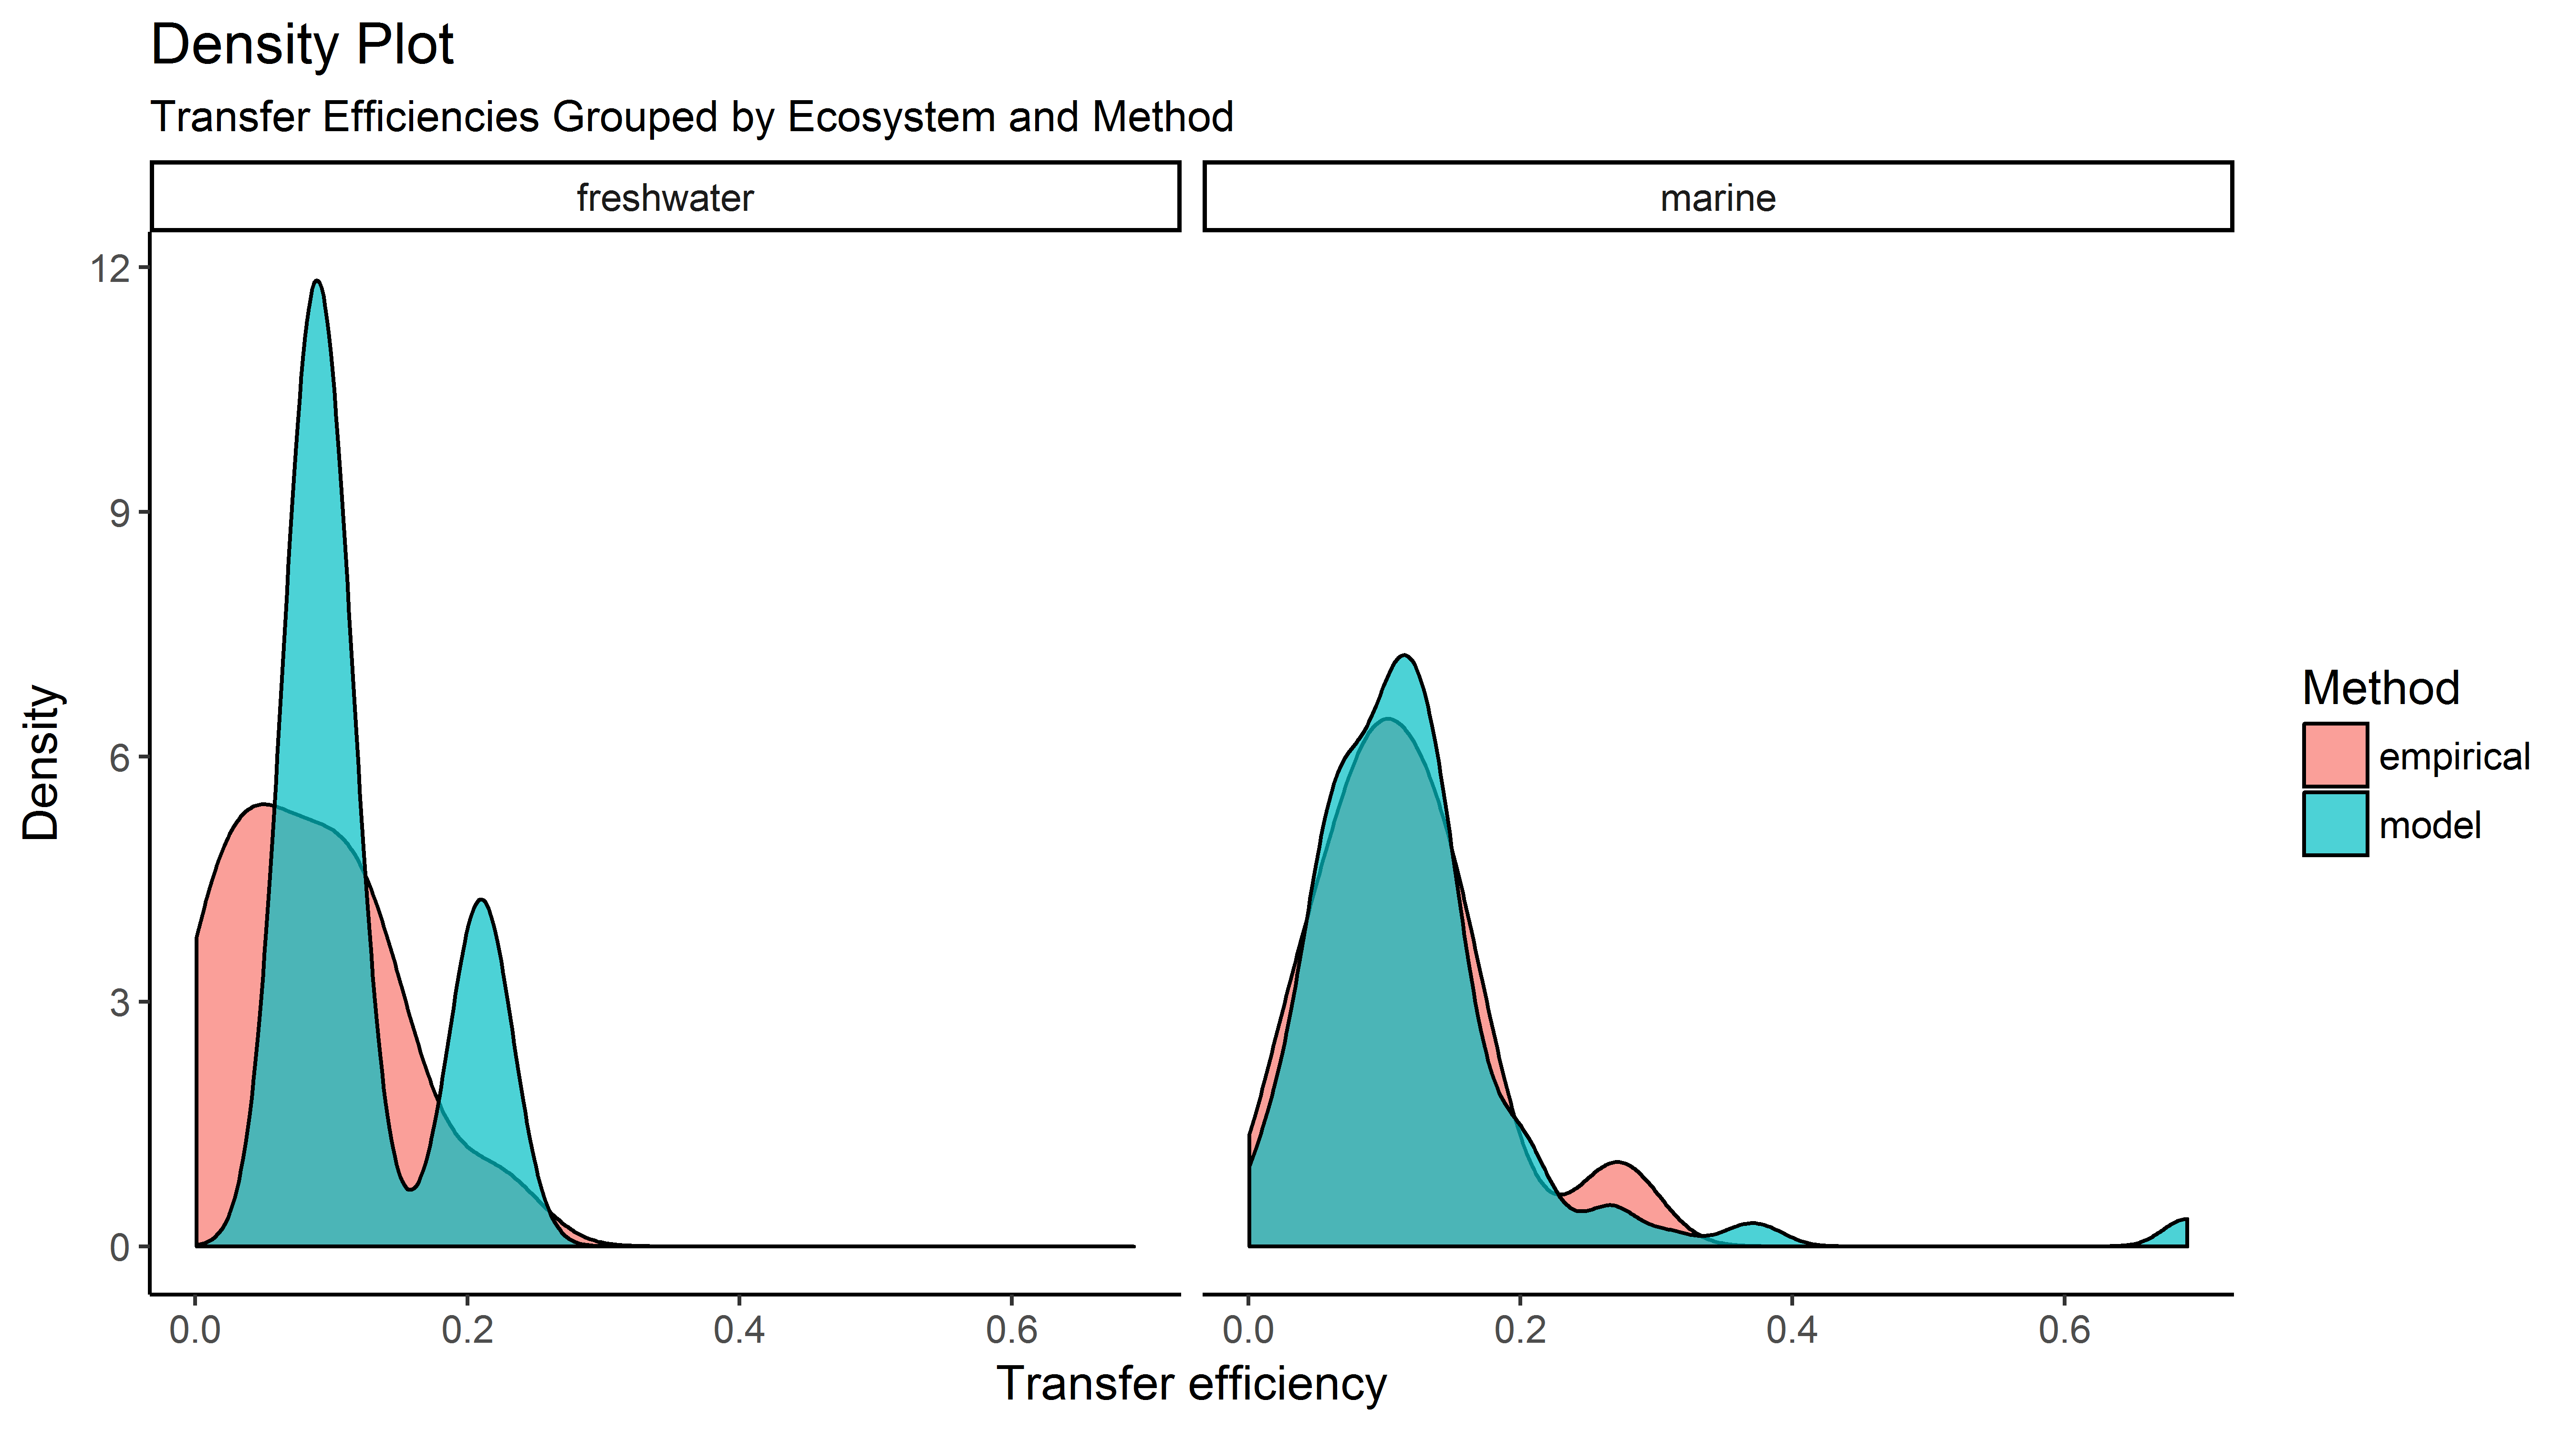
\includegraphics[width=\textwidth]{fig/density_eco_method}
    \caption{Density plot of transfer efficiencies where transfer efficiencies are grouped by ecosystem (i.e., freshwater vs. marine) and method (i.e., empirical and model-based).  There are a total of 15 transfer efficiency observations gathered from freshwater empirical studies, 4 observations from freshwater model-based studies, 13 from marine empirical studies, and 134 from marine model-based studies. Plot created using R v.3.4.3 \cite{Rcite} ggplot2 package v.2.2.1 \cite{ggplot}. }
    \label{dens_te}
\end{figure}

% Table generated by Excel2LaTeX from sheet 'Sheet1' with some big edits by Laura
%\begin{landscape}
\begin{longtable} {lp{3cm}p{2cm}lp{2cm}p{2cm}} 
	\toprule
    Articles & Region & Clustered Region & Method & Trophic Level & Transfer Efficiency \\
    \midrule
    Chea et al. 2016   & Tonle Sap Great Lake & lakes & model & average & 8.3 \\
    Gaedke 1993   & Lake Constance & lakes & model & average & 21 \\
    Lindeman 1942   & Cedar Bog Lake & lakes & empirical & producers & 0.1 \\
    Lindeman 1942   & Cedar Bog Lake & lakes & empirical & primary consumers & 13.3 \\
    Lindeman 1942   & Cedar Bog Lake & lakes & empirical & secondary consumers & 22.3 \\
    Lindeman 1942   & Lake Mendota & lakes & empirical & producers & 0.4 \\
    Lindeman 1942   & Lake Mendota & lakes & empirical & primary consumers & 8.7 \\
    Lindeman 1942   & Lake Mendota & lakes & empirical & secondary consumers & 5.5 \\
    Lindeman 1942   & Lake Mendota & lakes & empirical & tertiary consumers & 13 \\
    Odum 1959   & Silver Springs & springs & empirical & producers & 1.2 \\
    Odum 1959   & Silver Springs & springs & empirical & primary consumers & 16 \\
    Odum 1959   & Silver Springs & springs & empirical & secondary consumers & 11 \\
    Odum 1959   & Silver Springs & springs & empirical & tertiary consumers & 5 \\
    Rand and Stewart 1998   & Lake Michigan & lakes & empirical & tertiary consumers & 3.2 \\
    Rand and Stewart 1998   & Lake Ontario & lakes & empirical & primary consumers & 11.1 \\
    Rand and Stewart 1998   & Lake Ontario & lakes & empirical & secondary consumers & 8.3 \\
    Rand and Stewart 1998   & Lake Ontario & lakes & empirical & tertiary consumers & 4.6 \\
    Villaneuva et al. 2008   & Lake Kivu & lakes & model & average & 8.4 \\
    Villaneuva et al. 2006   & Lake Nokoue & lakes & model & average & 10.3 \\
    \bottomrule
    \caption{Freshwater transfer efficiency data}
         \label{datafresh}
    \end{longtable}
% \end{landscape}

\subsection*{Marine}
Marine studies on transfer efficiency did not commence until decades after the start of freshwater studies. The popularity of marine transfer efficiency research has increased rapidly in the past 20 years and has overall now exceeded the number of freshwater studies. A total of 115 sites have transfer efficiency data (Table \ref{datamar}). In contrast to the freshwater studies, most marine transfer efficiency data ($n=134$) come from model-based studies rather than empirical experiments ($n=13$). Most marine studies report the average value for an entire system ($n=94$). In studies that focused on individual transfer efficiencies between specific trophic levels, most focused on the transfer efficiency between phytoplankton (trophic level 1) and zooplankton (trophic level 2).

\vspace{5mm}

The empirical and model-based transfer efficiency data both form skewed-right distributions with large amounts of dispersion around the 10\% value (Figure \ref{dens_te}). For model-based observations, there are a few outlying points from a study on bays and estuaries that skew the distribution (Figure \ref{dens_te}). The combined transfer efficiency data ranges from 0.2\% to 69\% with a median of 10.6\%, while the range constricts with a minimum of 3.12\% to a maximum of 27.2\% for just the marine empirical studies (Figure \ref{dens_te}). 

\vspace{5mm}

To explore the potential drivers of variation in transfer efficiencies, we calculated importance plots from the decision tree analysis. When interpreting importance plots, the larger the score, the more influential the variable. A number close to zero indicates the variables is not important and could be dropped. When determining the importance of a variable, the mean decrease in accuracy (i.e., mean square error, MSE) or the mean decrease in node impurity are used to measure how well the trees split the data. Thus, the relative importance plots from the decision tree analysis indicate that trophic level had the greatest influence on transfer efficiency, followed by the clustered region (i.e., temperate shelves and seas, tropical shelves and seas, lagoons, upwelling ecosystems, and open oceans) (Figure \ref{varimp}). The method employed (i.e., empirical or model-based) did not appear to be a useful predictor.  

\begin{figure}[H]
     \centering
       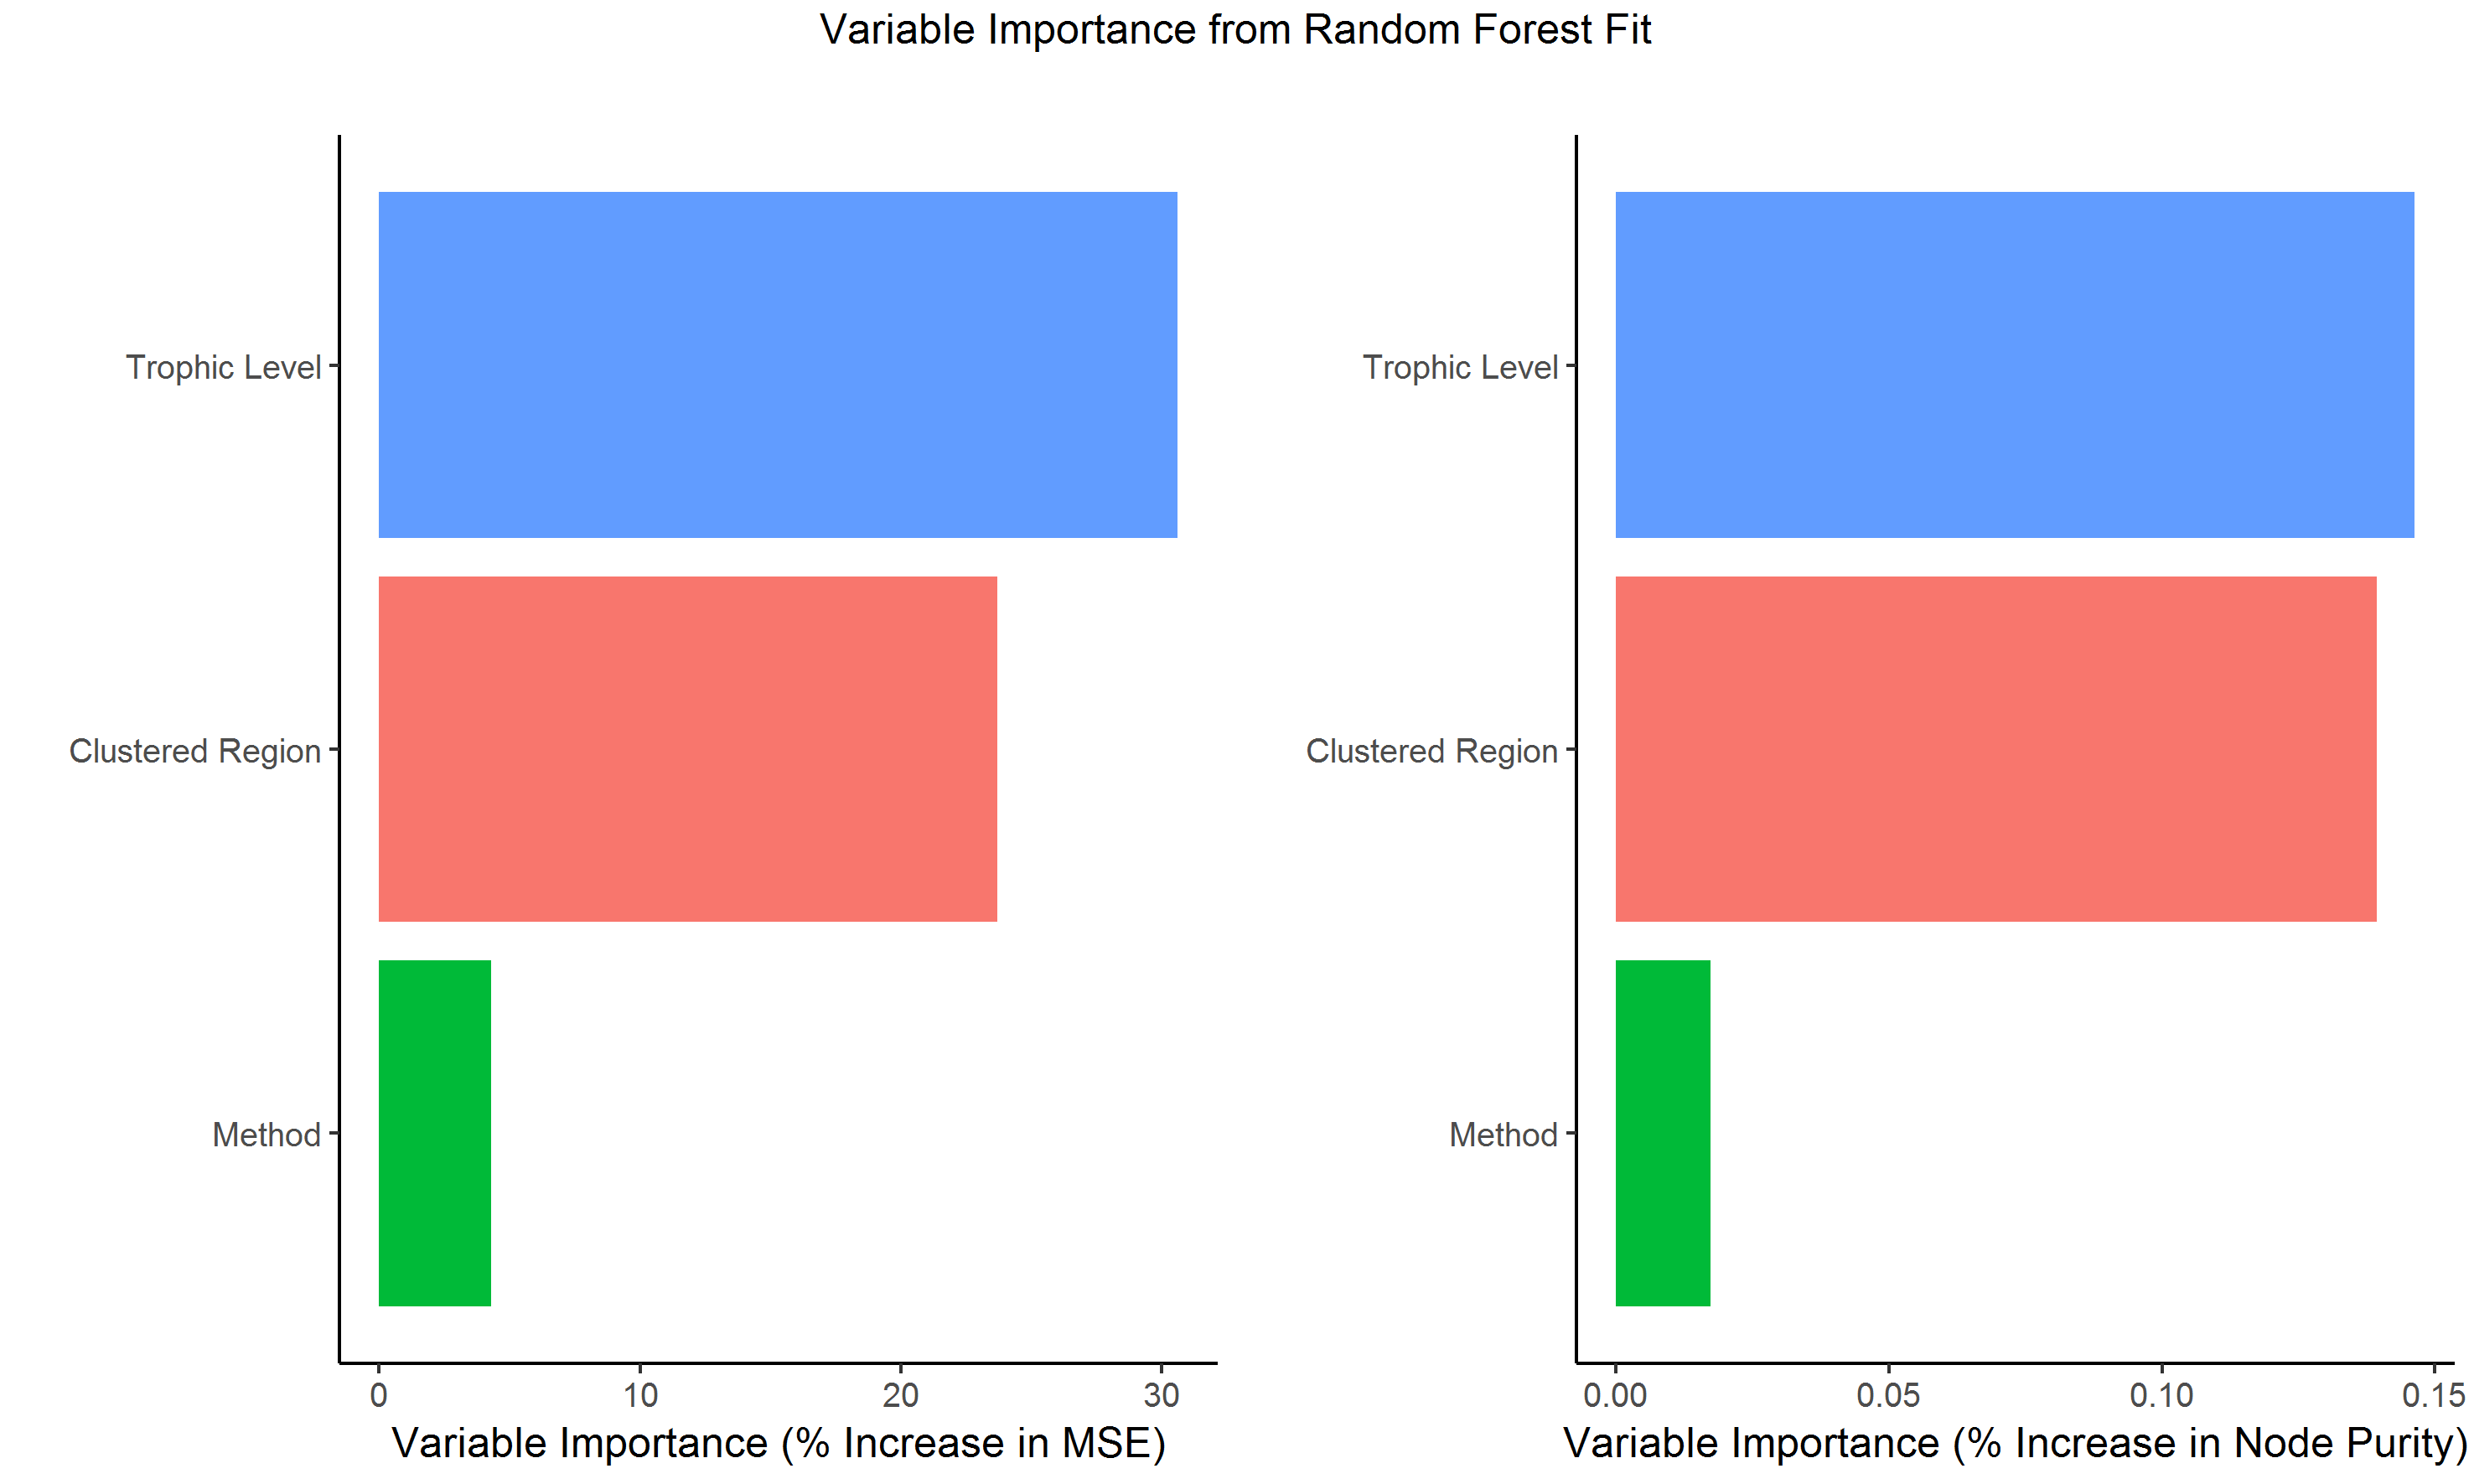
\includegraphics[width=\textwidth]{fig/var_imp_plot}
    \caption{Relative importance plots for random forest fit on marine transfer efficiency observations. In panel a), the predictors are ordered by percent increase in Mean Square Error (MSE). In panel b), the predictors are ordered by increase in node purity. Plot created using R v.3.4.3 \cite{Rcite} ggplot2 package v.2.2.1 \cite{ggplot}. }
    \label{varimp}
\end{figure}

We combined results across both marine and freshwater systems to examine differences among trophic levels (Figure 5). We combined data for all the systems to increase the sample size. Whether the different densities are due to the sensitivity to small samples sizes or systematic differences is unclear. Nonetheless, our results support the hypothesis that transfer efficiency decreases as trophic level increases (see \citealt{garcia2012reconsidering}). This in turn supports the results from  \citet{may1983ecology} that in the marine environment ectotherms (invertebrates then vertebrates), which dominate the lower trophic levels, are more efficient than endotherms, which are more prominent at higher trophic levels (Figure \ref{den_tl}). 

\begin{figure}[H]
     \centering
       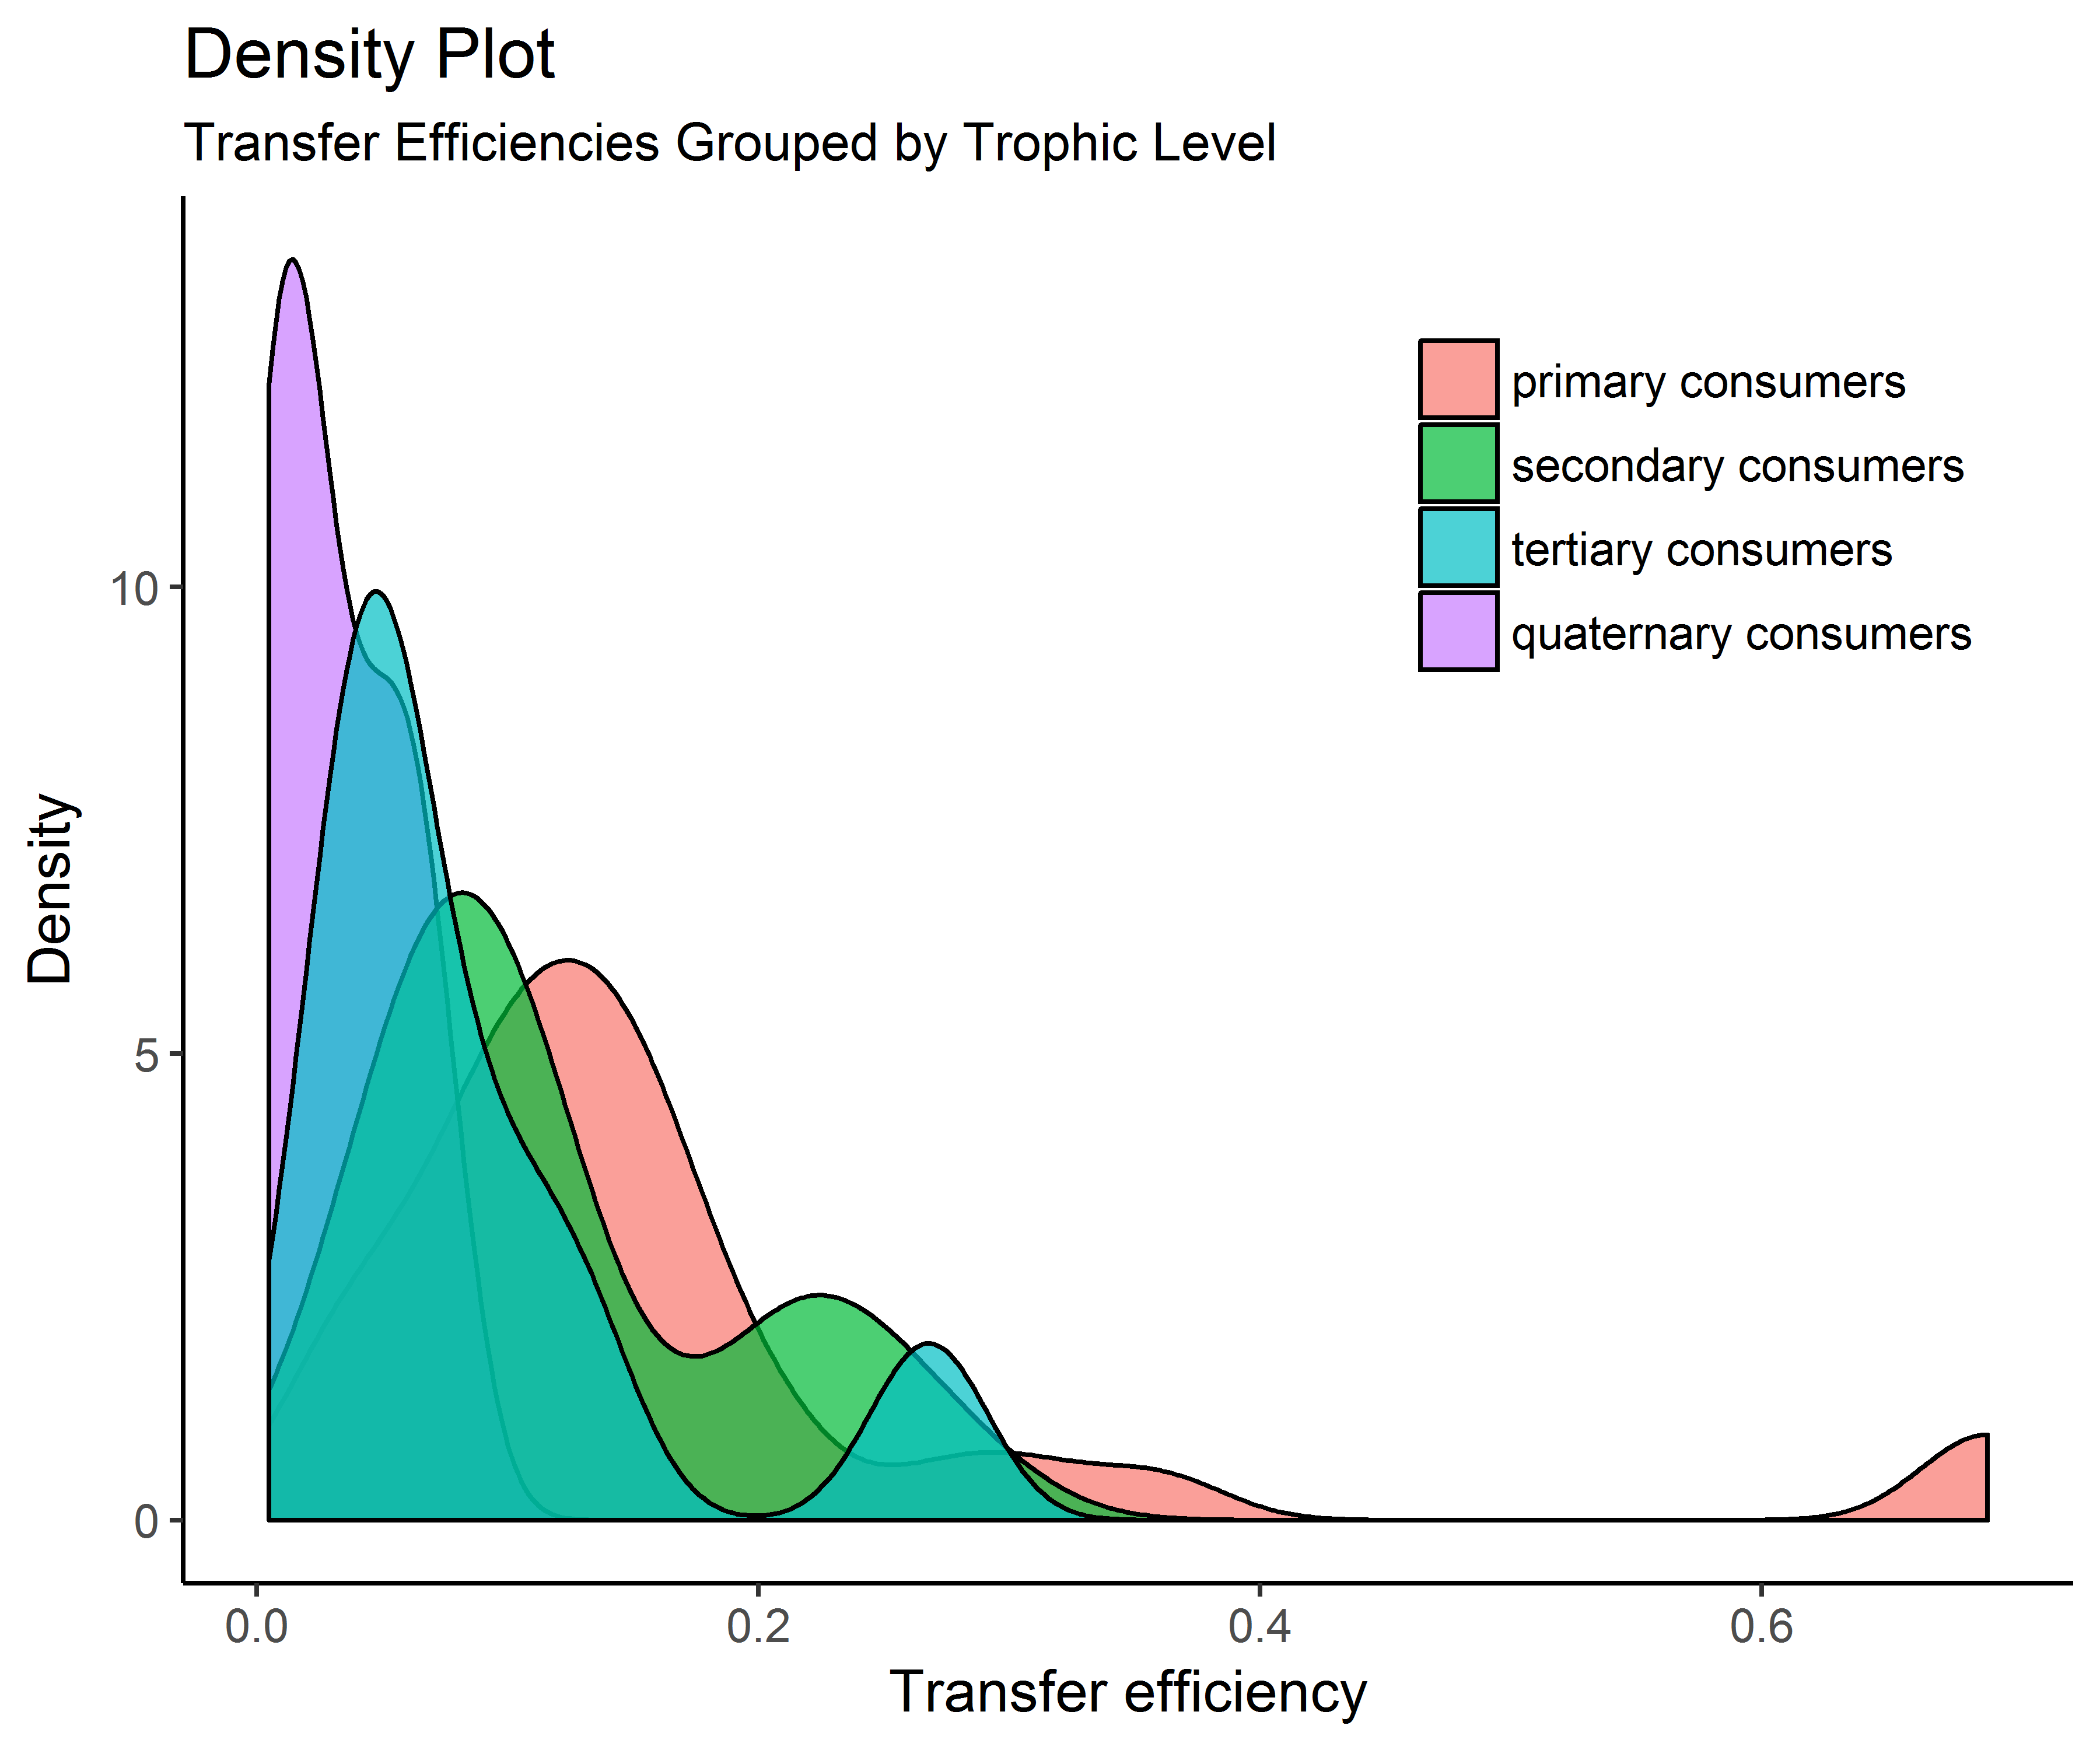
\includegraphics[width=.8\textwidth]{fig/density_te_by_tl}
    \caption{Density plot of transfer efficiencies grouped by trophic level. The data in this figure includes both ecosystem (i.e., freshwater and marine) and empirical and model-based transfer efficiency data. Plot created using R v.3.4.3 \cite{Rcite} ggplot2 package v.2.2.1 \cite{ggplot}. }
    \label{den_tl}
\end{figure}

% Table generated by Excel2LaTeX from sheet 'Sheet1' with some big edits by Laura
%\begin{landscape}
\begin{longtable} {p{4cm}p{3cm}p{2cm}lp{2cm}p{2cm}}
	\toprule
    Articles & Region & Clustered Region & Method & Trophic Level & Transfer Efficiency \\
    \midrule
    \endhead
    Akoglu et al. 2014  & Black Sea & temperate seas & model & primary consumers & 3 \\
    Akoglu et al. 2014   & Black Sea & temperate seas & model & secondary consumers & 3.8 \\
    Akoglu et al. 2014  & Black Sea & temperate seas & model & tertiary consumers & 7.4 \\
    Akoglu et al. 2014  & Black Sea & temperate seas & model & quaternary consumers & 0.5 \\
    Anjusha et al. 2013   & Gulf of Mannar & tropical seas & empirical & primary consumers & 13 \\
    Anjusha et al. 2013   & Gulf of Mannar & tropical seas & empirical & primary consumers & 12 \\
    Anjusha et al. 2013   & Gulf of Mannar & tropical seas & empirical & primary consumers & 14.6 \\
    Anjusha et al. 2013  & Gulf of Mannar & tropical seas & empirical & primary consumers & 9.1 \\
    Anjusha et al. 2013   & Gulf of Mannar & tropical seas & empirical & primary consumers & 6.8 \\
    Anjusha et al. 2013 & Palk Bay & tropical seas & empirical & primary consumers & 27.2 \\
    Anjusha et al. 2013   & Palk Bay & tropical seas & empirical & primary consumers & 17.6 \\
    Anjusha et al. 2013  & Palk Bay & tropical seas & empirical & primary consumers & 9.39 \\
    Anjusha et al. 2013  & Palk Bay & tropical seas & empirical & primary consumers & 7.19 \\
    Anjusha et al. 2013  & Palk Bay & tropical seas & empirical & primary consumers & 3.12 \\
    Anjusha et al. 2013  & Palk Bay & tropical seas & empirical & primary consumers & 3.23 \\
    Baird et al. 2004  & Sylt-Romo Bight & temperate seas & model & average & 2.61 \\
    Baird et al. 2007  & Sylt-Romo Bight: arenicola flats & temperate seas & model & average & 3.47 \\
    Baird et al. 2007  & Sylt-Romo Bight: dense zostera noltii beds & temperate seas & model & average & 5.58 \\
    Baird et al. 2007  & Sylt-Romo Bight: mud flats & temperate seas & model & average & 6.13 \\
    Baird et al. 2007   & Sylt-Romo Bight: muddy sand flats & temperate seas & model & average & 7.31 \\
    Baird et al. 2007   & Sylt-Romo Bight: mussel beds & temperate seas & model & average & 14.92 \\
    Baird et al. 2007  & Sylt-Romo Bight: pelagic domain & temperate seas & model & average & 1 \\
    Baird et al. 2007  & Sylt-Romo Bight: sandy beaches & temperate seas & model & average & 6.5 \\
    Baird et al. 2007  & Sylt-Romo Bight: sandy shoals & temperate seas & model & average & 3.3 \\
    Baird et al. 2007   & Sylt-Romo Bight: sparse zostera noltii beds & temperate seas & model & average & 5.06 \\
    Barnes et al.  2010  & summary of 21 locations & -    & model & average small sizes & 13.8 \\
    Barnes et al.  2010   & summary of 21 locations & -    & model & average large sizes & 5.8 \\
    Baumann 1995   & general claim & -    & empirical & average & 15 \\
    Bradford-Grieve et al. 2003   & Southern Plateau, New Zealand & temperate seas & model & secondary consumers & 23 \\
    Chassot et al. 2010  & temperate & temperate seas & model & average & 10 \\
    Chassot et al. 2010   & tropical & tropical seas & model & average & 14 \\
    Chassot et al. 2010  & upwelling & upwelling ecosystems & model & average & 5 \\
    Cornejo-Donoso and Antezana 2008   & Antarctic Peninsula & temperate seas & model & primary consumers & 21 \\
    Cornejo-Donoso and Antezana 2008  & Antarctic Peninsula & temperate seas & model & secondary consumers & 20 \\
    Cornejo-Donoso and Antezana 2008  & Antarctic Peninsula & temperate seas & model & tertiary consumers & 10 \\
    Cornejo-Donoso and Antezana 2008   & Antarctic Peninsula & temperate seas & model & quaternary consumers & 5 \\
    D'Alelio et al. 2016   & Gulf of Naples & temperate seas & model & primary consumers & 20 \\
    Duan et al. 2009  & Pearl River Estuary & tropical seas & model & average & 10.2 \\
    Gamito and Erzini 2004  & Ria Formosa lagoon, south Portugal & lagoons & model & primary consumers & 4.8 \\
    Gamito and Erzini 2004   & Ria Formosa lagoon, south Portugal & lagoons & model & secondary consumers & 6 \\
    Gamito and Erzini 2004   & Ria Formosa lagoon, south Portugal & lagoons & model & tertiary consumers & 3.5 \\
    Gamito and Erzini 2004   & Ria Formosa lagoon, south Portugal & lagoons & model & quaternary consumers & 1.2 \\
    Gamito and Erzini 2004   & Ria Formosa lagoon, south Portugal & lagoons & model & quinary consumers & 0.2 \\
    Libralto et al. 2008   & Atlantic coast of Morocco  & temperate seas & model & average & 10.9 \\
    Libralto et al. 2008   & Azores archipelago & temperate seas & model & average & 10.5 \\
    Libralto et al. 2008   & Bali Strait & tropical seas & model & average & 11.7 \\
    Libralto et al. 2008   & Baltic sea & temperate seas & model & average & 25.9 \\
    Libralto et al. 2008  & Bay of Bengal & tropical seas & model & average & 9 \\
    Libralto et al. 2008   & Bay of Biscay & temperate seas & model & average & 16.5 \\
    Libralto et al. 2008   & Bay of Revellata, Corsica & temperate seas & model & average & 18.8 \\
    Libralto et al. 2008   & Bolinao reef flat & tropical seas & model & average & 10.4 \\
    Libralto et al. 2008   & Brunei Darussalam & tropical seas & model & average & 12.9 \\
    Libralto et al. 2008  & California upwelling & upwelling ecosystems & model & average & 4 \\
    Libralto et al. 2008  & Campeche Bank of Yucatan shelf & tropical seas & model & average & 17.6 \\
    Libralto et al. 2008   & Cantabric Sea & temperate seas & model & average & 38.1 \\
    Libralto et al. 2008  & Celestun lagoon, Mexico & lagoons & model & average & 6.4 \\
    Libralto et al. 2008   & Central North Pacific Ocean & temperate seas & model & average & 4.4 \\
    Libralto et al. 2008   & Chesapeake Bay & temperate seas & model & average & 12.5 \\
    Libralto et al. 2008  & Chiku lagoon, Taiwan & lagoons & model & average & 13.1 \\
    Libralto et al. 2008  & Coast of Western Gulf of Mexico & tropical seas & model & average & 16.2 \\
    Libralto et al. 2008  & Coastal areas and reefs & -    & model & average & 13 \\
    Libralto et al. 2008  & Continental shelf of southern Brazil & tropical seas & model & average & 11.8 \\
    Libralto et al. 2008   & Eastern Bering Sea & temperate seas & model & average & 13.2 \\
    Libralto et al. 2008   & Eastern Scotian shelf & temperate seas & model & average & 11 \\
    Libralto et al. 2008   & Eastern Tropical Pacific Ocean & temperate seas & model & average & 20.4 \\
    Libralto et al. 2008  & Etang de Thau, France  & lagoons & model & average & 10.8 \\
    Libralto et al. 2008   & Faroe Islands & temperate seas & model & average & 14.4 \\
    Libralto et al. 2008  & Faroe Islands & temperate seas & model & average & 15.4 \\
    Libralto et al. 2008  & Floreana rocky reef Galapagos & tropical seas & model & average & 13 \\
    Libralto et al. 2008  &  Georgia Strait & temperate seas & model & average & 9.5 \\
    Libralto et al. 2008   & Great Barrier Reef & tropical seas & model & average & 11.5 \\
    Libralto et al. 2008  & Gulf of Lingayen & tropical seas & model & average & 13.5 \\
    Libralto et al. 2008   & Gulf of Maine - Georges Bank & temperate seas & model & average & 15.6 \\
    Libralto et al. 2008   & Gulf of Mexico continental shelf  & tropical seas & model & average & 9.7 \\
    Libralto et al. 2008  & Gulf of Thailand & tropical seas & model & average & 10.4 \\
    Libralto et al. 2008  & Hong Kong & tropical seas & model & average & 9.1 \\
    Libralto et al. 2008   & Icelandic fisheries & temperate seas & model & average & 14.2 \\
    Libralto et al. 2008   & Kuala Trengganu & tropical seas & model & average & 17.8 \\
    Libralto et al. 2008   & Laguna de Bay, Philippines & lagoons & model & average & 12.4 \\
    Libralto et al. 2008  & Lancaster Sound Region & temperate seas & model & average & 8.2 \\
    Libralto et al. 2008   & Maputo Bay & temperate seas & model & average & 7.6 \\
    Libralto et al. 2008   & Newfoundland & temperate seas & model & average & 14.3 \\
    Libralto et al. 2008  &  North Benguela upwelling & upwelling ecosystems & model & average & 7.9 \\
    Libralto et al. 2008 & North Coast of Central Java & tropical seas & model & average & 11.8 \\
    Libralto et al. 2008   & North Sea & temperate seas & model & average & 11.6 \\
    Libralto et al. 2008  & Northern British Columbia & temperate seas & model & average & 14.2 \\
    Libralto et al. 2008   & Northern Gulf of Saint Lawrence  & temperate seas & model & average & 12 \\
    Libralto et al.  2008   & Northern-central Adriatic Sea  & temperate seas & model & average & 10 \\
    Libralto et al. 2008  & Norwegian and Barents Sea & temperate seas & model & average & 10.5 \\
    Libralto et al. 2008  & NW Africa upwelling & upwelling ecosystems & model & average & 6.1 \\
    Libralto et al. 2008  & Open oceans & open oceans & model & average & 12 \\
    Libralto et al. 2008   & Orbetello lagoon & lagoons & model & average & 9.6 \\
    Libralto et al. 2008   & Peru upwelling & upwelling ecosystems & model & average & 6.6 \\
    Libralto et al. 2008   & Prince William Sound, Alaska & temperate seas & model & average & 14.1 \\
    Libralto et al. 2008  & San Miguel Bay & tropical seas & model & average & 20.6 \\
    Libralto et al. 2008  & San Pedro Bay & tropical seas & model & average & 9.4 \\
    Libralto et al. 2008   & Schlei Fjord & temperate seas & model & average & 7.4 \\
    Libralto et al. 2008   & Shallow areas of Gulf of Thailand & tropical seas & model & average & 6.8 \\
    Libralto et al. 2008   & South Catalan Sea & temperate seas & model & average & 12.6 \\
    Libralto et al. 2008   & South China Deep Sea & tropical seas & model & average & 10.6 \\
    Libralto et al. 2008   & Southern Brazil & tropical seas & model & average & 6.3 \\
    Libralto et al. 2008   & Southwest coast of India & tropical seas & model & average & 14 \\
    Libralto et al. 2008  & Tampa Bay & tropical seas & model & average & 8.6 \\
    Libralto et al. 2008  & Temperate shelves & temperate seas & model & average & 14 \\
    Libralto et al. 2008   & Tropical shelves & tropical seas & model & average & 10 \\
    Libralto et al. 2008   & Upwellings & upwelling ecosystems & model & average & 5 \\
    Libralto et al. 2008   & Venezuela northeastern shelf & tropical seas & model & average & 7.3 \\
    Libralto et al. 2008   & Venice lagoon & lagoons & model & average & 14.5 \\
    Libralto et al. 2008   & Vietnam-China shelf & tropical seas & model & average & 7.5 \\
    Libralto et al. 2008   & West Coast of Vancouver Island & temperate seas & model & average & 13.7 \\
    Libralto et al. 2008   & West Greenland  coast & temperate seas & model & average & 12.1 \\
    Libralto et al. 2008   & West Greenland trawling area & temperate seas & model & average & 7.1 \\
    Lin et al. 2006  &  Tapong Bay, southwestern Taiwan & tropical seas & model & average & 5.5 \\
    Liu et al. 2009  &  Nanwan Bay, southern Taiwan & tropical seas & model & primary consumers & 13.9 \\
    Liu et al. 2009  &  Nanwan Bay, southern Taiwan & tropical seas & model & secondary consumers & 6.6 \\
    Liu et al. 2009  & Nanwan Bay, southern Taiwan & tropical seas & model & tertiary consumers & 5.2 \\
    Liu et al. 2009   & Nanwan Bay, southern Taiwan & tropical seas & model & quaternary consumers & 2 \\
    Manickchand-Heileman et al. 2003   & Gulf of Paria, Venezuela and Trinidad & tropical seas & model & average & 12.2 \\
    Neira and Arancibia 2004   & upwelling Central Chile & upwelling ecosystems & model & primary consumers & 8.1 \\
    Neira and Arancibia 2004  & upwelling Central Chile & upwelling ecosystems & model & secondary consumers & 27.4 \\
    Neira and Arancibia 2004   & upwelling Central Chile & upwelling ecosystems & model & tertiary consumers & 26.8 \\
    Neira and Arancibia 2004   & upwelling Central Chile & upwelling ecosystems & model & quaternary consumers & 6.7 \\
    Neira and Arancibia 2004   & upwelling Central Chile & upwelling ecosystems & model & quinary consumers & 7.4 \\
    Pauly and Christensen 1995   & general claim & NA    & empirical & average & 10.13 \\
    Rybarczyk and Elkaim 2003   & Bay of Somme & temperate seas & model & primary consumers & 15.6 \\
    Rybarczyk and Elkaim 2003   & Chesapeake Bay & temperate seas & model & primary consumers & 31 \\
    Rybarczyk and Elkaim 2003  & Delaware Bay & temperate seas & model & primary consumers & 69 \\
    Rybarczyk and Elkaim 2003   & Narragansett Bay & temperate seas & model & primary consumers & 69 \\
    Rybarczyk and Elkaim 2003   & Seine Estuary & temperate seas & model & primary consumers & 36.05 \\
    Sheldon et al. 1977  &  ocean pelagic & open oceans & model & primary consumers & 15 \\
    Tsagarakis et al. 2010  & N. Aegean & temperate seas & model & average & 17.4 \\
    Tsagarakis et al. 2010  & N.C. Adriatic  & temperate seas & model & average & 10 \\
    Tsagarakis et al. 2010   & S. Catalan & temperate seas & model & average & 12.6 \\
    Villaneuva et al. 2006  & Ebrie lagoon  & lagoons & model & average & 15.5 \\
    Ware 2000  & Georges Bank & temperate seas & model & primary consumers & 15.9 \\
    Ware 2000   & Gulf of Maine & temperate seas & model & primary consumers & 11.9 \\
    Ware 2000  & Gulf of Maine & temperate seas & model & secondary consumers & 10.5 \\
    Ware 2000  & Mid-Atlantic Shelf & tropical seas & model & primary consumers & 10.2 \\
    Ware 2000   & Mid-Atlantic Shelf & tropical seas & model & secondary consumers & 10.1 \\
    Ware 2000   & Nova Scotia Shelf & temperate seas & model & primary consumers & 12.1 \\
    Ware 2000   & Nova Scotia Shelf & temperate seas & model & secondary consumers & 12.3 \\
    Ware 2000   & Oyashio current model & temperate seas & model & primary consumers & 17 \\
    Ware 2000   & Oyashio current model & temperate seas & model & secondary consumers & 7.9 \\
    Ware 2000   & SW Britisth Columbia model & temperate seas & model & primary consumers & 11.1 \\
    Ware 2000   & SW Britisth Columbia model & temperate seas & model & secondary consumers & 8 \\
    \bottomrule
    \caption{Marine transfer efficiency data}
    \label{datamar}
    \end{longtable}
% \end{landscape}


\section*{Discussion}
Overall, these studies show similarities between the two systems. The results give visual evidence that although the average transfer efficiency does not differ greatly from 10\%, there is substantial variation in transfer efficiency in both systems (Figure \ref{dens_te}). Additionally our study was able to identify that trophic level and the general geographic location of the ecosystem impacts the variability of the transfer efficiency. Some of this large variation seems to have predictable patterns, but the potential sources of this variation can only be explored for the larger sample sizes from marine systems. Thus in the absence of data, the distributions generated in the current study are good starting points to model the variation in transfer efficiency. 

\vspace{5mm}

We hypothesize the difference in transfer efficiency between trophic levels could be partially attributed to the composition of the taxa. Additionally, the differences could be due to the mobility of the organisms at each trophic levels and the amount of energy expedited to capture their prey. Both of these points highlight the need for additional research that can distinguish between the different mechanisms that influence transfer efficiency (e.g., endotherms vs. ectotherms).

\vspace{5mm}

We encountered two main difficulties in this study due to the different naming conventions in the early states (Figure \ref{foodweb} and \ref{flowchart}) and the different efficiencies of interest amongst different fields. We bring this point up to highlight the challenges in conducting interdisciplinary work. We found freshwater studies report either assimilation and consumption efficiencies or transfer efficiency, while the majority of marine papers focused on transfer efficiency. As previously mentioned, we found very few terrestrial studies that reported results on transfer efficiency. It is intriguing that the focus on transfer efficiency is an aquatic phenomenon. While we are unable to say with certainty why this is, we can speculate that in aquatic systems, and especially marine systems, it is extremely difficult to gather data on most species in an ecosystem. As a result, it is challenging to calculate the assimilation and consumption efficiencies in these systems. The great ease in counting terrestrial populations means the studies do not need to rely on more inferential, trophic level wide, techniques.

\vspace{5mm}

Despite the aforementioned limitations, we are able to demonstrate the 10\% value is problematic given the substantial variation that exists in the transfer efficiency. Even though the average and median values that emerge from the synthesis are not dramatically different from 10\%--which may suggest that an assumption of 10\% would be reasonable--by continuing to use a 10\% transfer efficiency researchers are eschewing the large variation and predictable patterns within this variation, which will impact a food web model?s ability to provide realistic results. From here on, we explore implications of applying a fixed 10\% transfer efficiency in ecology, fisheries, and aquaculture.

\subsection*{Applications in ecology}
When it comes to ecology, the transfer efficiency is used to understand food web dynamics and how various species interact and influence one another. Most commonly, it is used in size spectrum studies that explore predator-prey relationships \cite{barnes2010global}. In general though, the more detailed and species-specific assimilation efficiency is used more frequently in such analyses. Since many issues within ecology and conservation biology focus on individual species patterns, it is valuable to be able to calculate species-specific efficiencies. The transfer efficiency is perhaps too broad of a metric for many questions. While using a 10\% transfer efficiency value can have drastic underrepresentation and lead to severely mismanaged systems, given the preference for the assimilation efficiency the implications of a 10\% transfer efficiency most likely has not been directly measured in many cases in ecology. Previous research has shown distinct transfer efficiencies between trophic levels and for terrestrial (i.e., temperate forests, deciduous forests, and grasslands) and freshwater (i.e., lakes) systems \cite{hairston1993causeeffect}. Even though the assimilation and consumption efficiencies are different measures, there is comparable variation in them as there is in the transfer efficiency data, and therefore the implications of applying fixed values for these efficiencies could be the same as those for the transfer efficiency.

\subsection*{Applications in fisheries}
In fisheries, transfer efficiency is mostly used to determine the impact of fishing on a population. It can be used to estimate various metrics, such as biomass and the primary production required (PPR) given fisheries catch. Primary production required estimates the amount of net primary production needed to replace the biomass removed by fisheries landings. The idea is that primary production is a major limiting factor of fisheries catch. If biomass or the primary production required is incorrectly estimated, we risk the potential of under- or overfishing. 

\vspace{5mm}

What is the cost of ignoring variability in transfer efficiencies for fisheries applications? To explore this question, we reexamined the analyses by \citet{chassot2010global} and \citet{watson2014primary} of the primary production required to produce the biomass of fish that were caught. As an exploration, we recreated the analysis for one marine region, the California Current. We gathered annual catch data from Sea Around Us (\url{http://www.seaaroundus.org/}) from 1950 to 2014, trophic level data on fishes from Fishbase data base (\url{http://www.fishbase.org/}), and net primary production data on SeaWiFS from the Ocean Productivity web site (\url{http://www.science.oregonstate.edu/ocean.productivity/}). \citet{watson2014primary} also included trophic level data on invertebrates from SeaLifeBase; however, SeaLifeBase does not include trophic level data for the California Current. We first replicated the previously published results using a fixed 10\% transfer efficiency using the following equation\footnote{\citet{chassot2010global} specified ecosystem specific transfer efficiencies.}.

\begin{equation}
PPR_t = \sum_{i=1}^{n}\frac{C_{i,t}}{CR}*\frac{1}{TE}^{TL_i-1}
\end{equation}

$PPR_t$ is the primary production required in year $t$ to produce the observed catch, $C_{i,t}$ is the biomass of catch for species $i$ in year $t$, $CR$ is the conversion rate of carbon to wet weight, $TE$ is the transfer efficiency, $TL_i$ is trophic level for species $i$, and $n$ is the number of species within a region. 

\vspace{5mm}

To explore the impact of ignoring variability in transfer efficiencies, we used the data we gathered on marine transfer efficiencies to test for sensitivities to transfer efficiency variability. We fit an approximate distribution to the marine transfer efficiency data using goodness-of-fit criterion so that we could randomly sample a value from the observed distribution instead of using a fixed 10\% value in the above equation (See supporting information for details). This approach allowed us to incorporate variability in the transfer efficiency. While the time span of the Sea Around Us catch data ran for over 60 years, we explored the distribution at 20 year intervals to get a sample of the changes in transfer efficiency. We constructed Monte Carlo simulations and ran 10,000 simulations for the years 1950, 1970, 1990, and 2010. Although it is difficult to compare our results directly to \citet{watson2014primary}, since their results are broken up by continental fishing fleets, we found that when transfer efficiency is allowed to vary, the projected PPR varies dramatically. Although the majority of the time the PPR is a sustainable fraction of the total production of the California Current, on average 47.18\% of the time (i.e., 46.93\% in 1950, 47.21\% in 1970, 47.35\% in 1990, and 47.22\% in 2010) the simulations suggest annual landings could exceed total primary production (Figure \ref{ppr}). Therefore, the application of a 10\% transfer efficiency in fisheries management has a high chance of leading to unsustainable fishing practices. 

\begin{figure}[H]
     \centering
       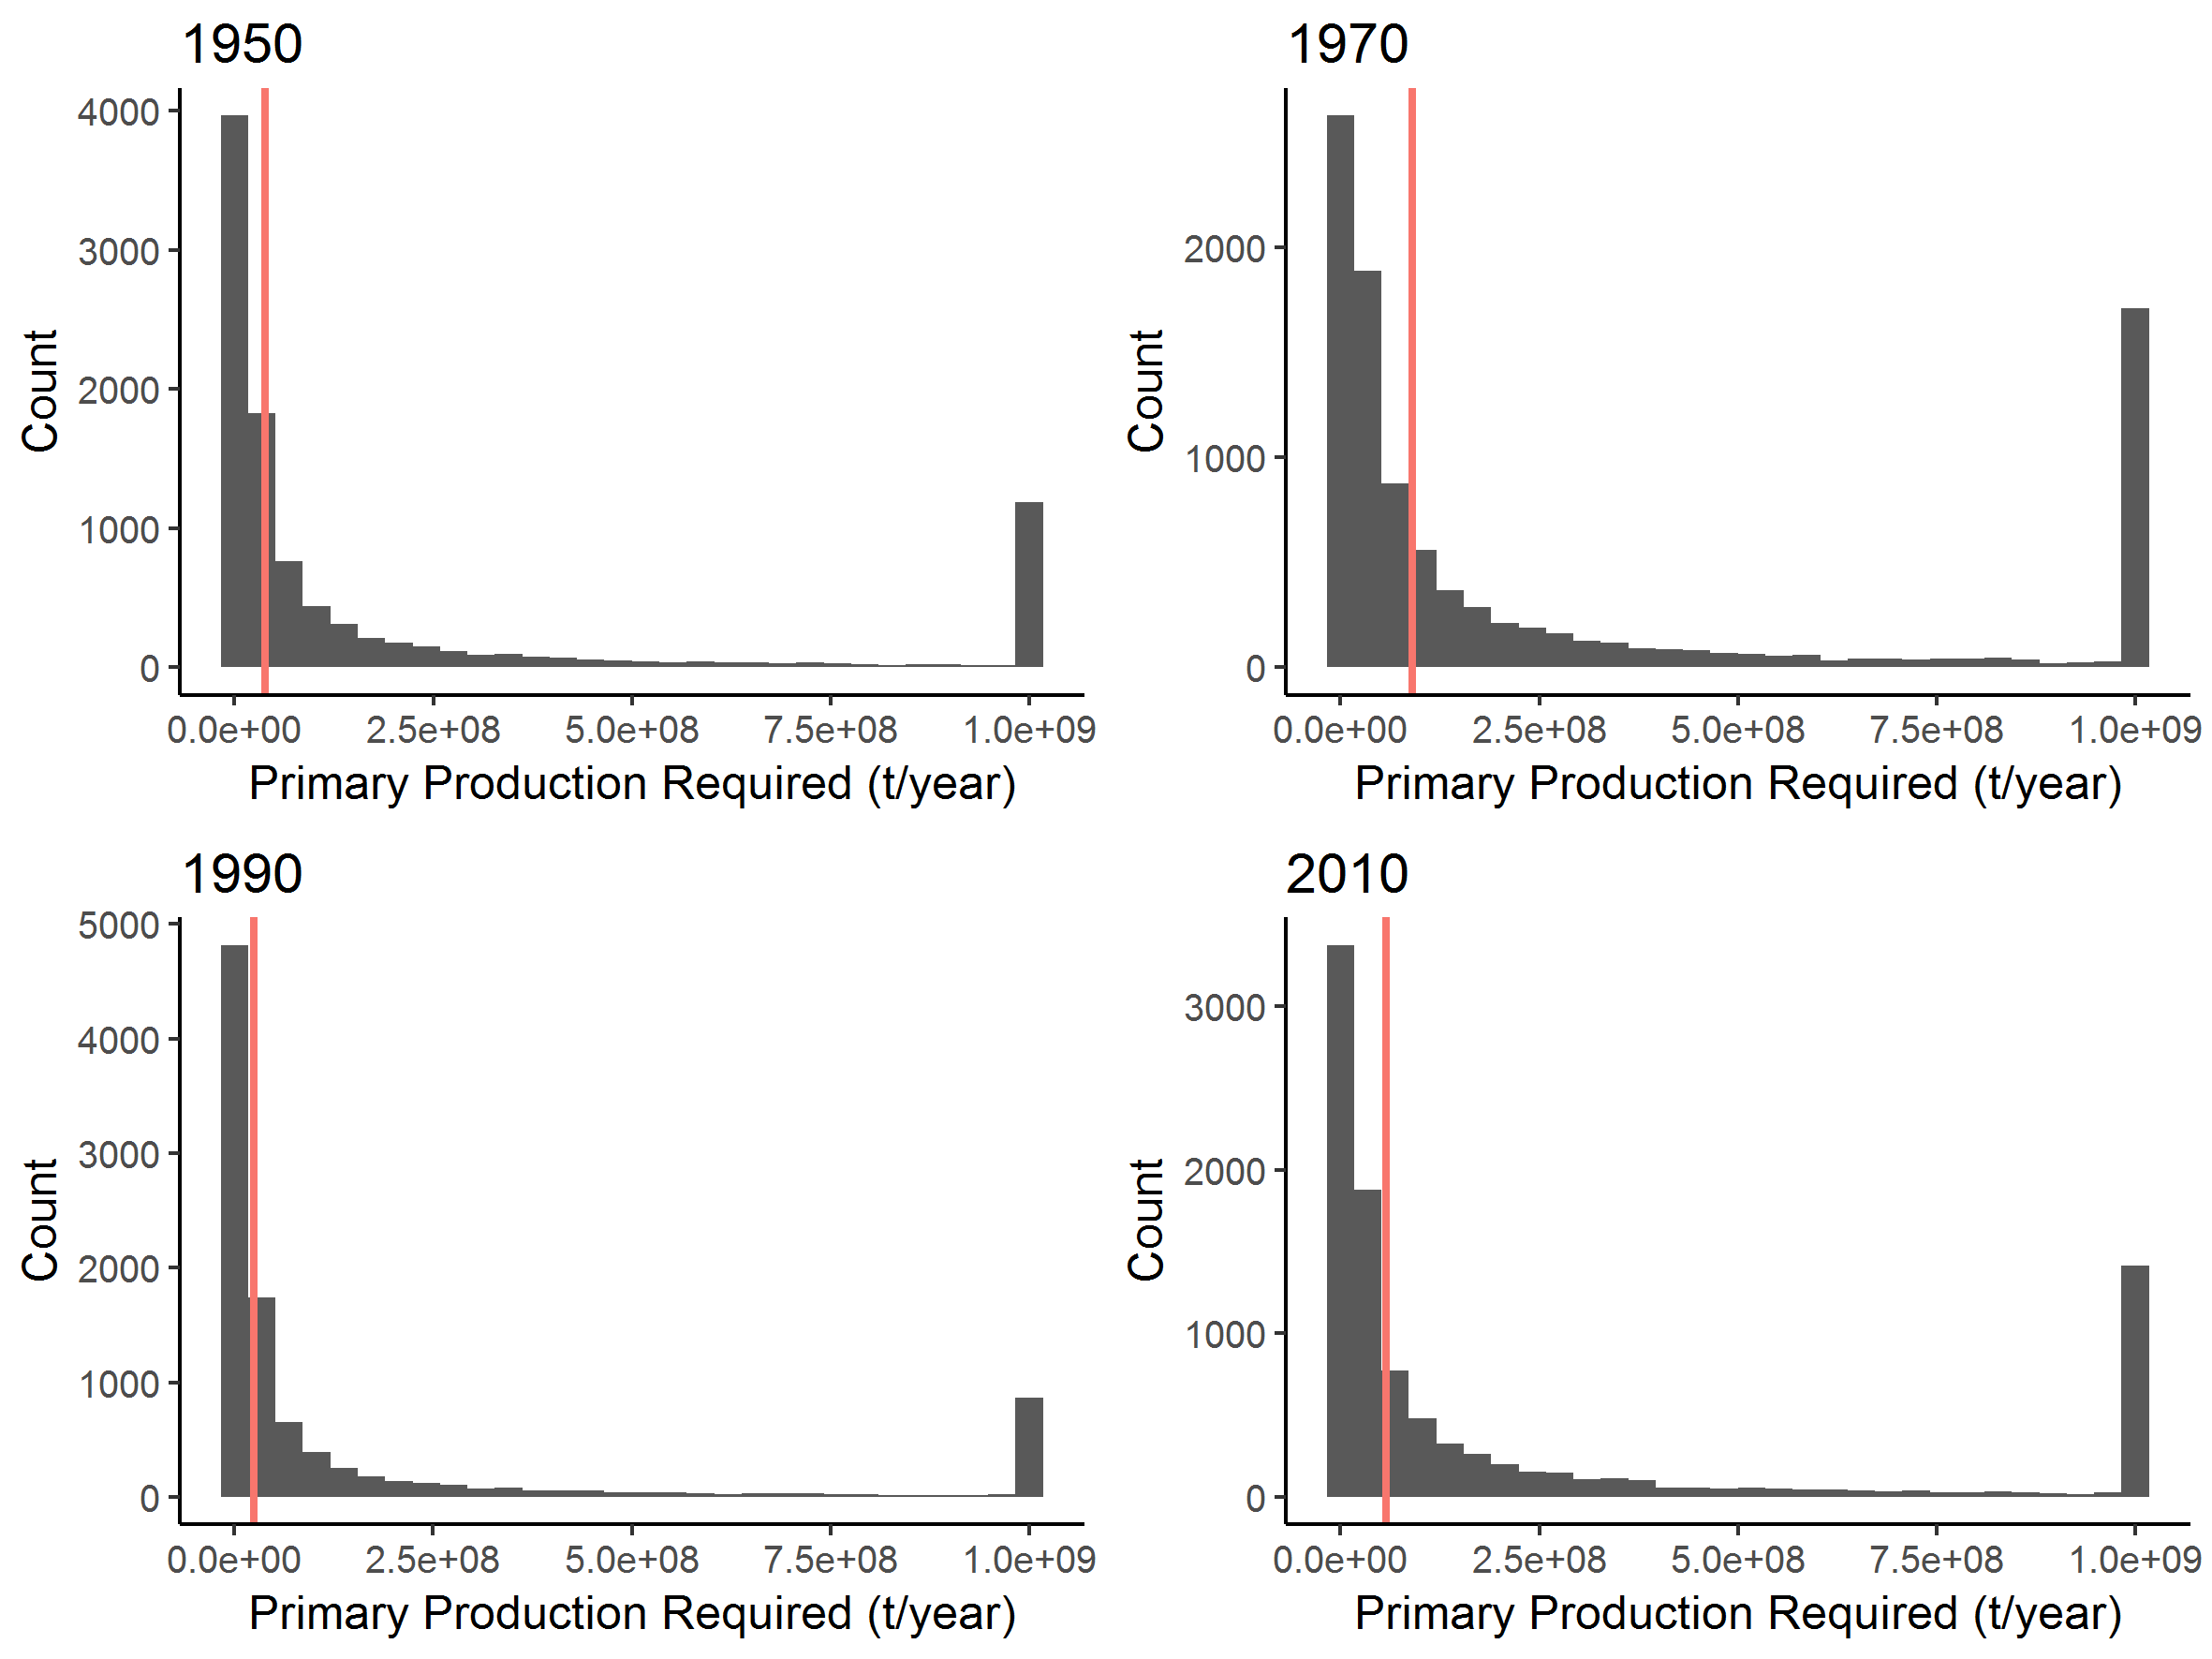
\includegraphics[width=.8\textwidth]{fig/hist_ppr_1950_2010}
    \caption{Histogram of simulated primary production required given catch divided by the average primary production in 1950, 1970, 1990, and 2010 in the California Current using a random transfer efficiency. The vertical red line indicates the primary production required divided by primary production using a fixed 10\% transfer efficiency in the calculations. We adjusted the far right bin width due to rare events. The original range extends out further. Plot created using R v.3.4.3 \cite{Rcite} ggplot2 package v.2.2.1 \cite{ggplot}. }
    \label{ppr}
\end{figure}

\subsection*{Applications in aquaculture}
Aquaculture already cultivates hundreds of different marine and freshwater species. The relevance of transfer efficiencies to production decisions depends on whether the species requires additional feed or not. Non-fed aquaculture includes either primary producers or primary consumers that are not provided additional feeds by the aquaculturist. Fed aquaculture, on the other hand, involves consumer species that are typically fed compound feeds designed to meet their specific nutritional requirements. Consumption of autotrophs, usually phytoplankton by filter feeders, is studied extensively in non-fed aquaculture to track carrying capacity of ecosystems with added aquaculture \cite{banas2007tidal}. These carrying capacities are estimated using assimilation efficiencies of a specific target species \cite{rosland2009applying, irisarri2013absorption, srisunont2016estimating} or as broader estimates of transfer efficiencies \cite{simenstad1995influence, sommer1998algal, byron2011calculating, han2017evaluating}.

\vspace{5mm}

More and more fed species are given specialized compound feeds rather than whole organisms in order to increase efficiency and sustainability of feed resources. To assess the sustainability of feeds, the field has begun to track transfer efficiencies by dissecting the feed into its compositional parts and estimating the efficiencies for each of the components using the method devised by \citet{pauly1995primary}. While a 10\% transfer efficiency was initially employed to estimate the primary production requirements or biotic resource use in environmentally-based aquaculture assessments (e.g., \citealt{papatryphon2004environmental, pelletier2007feeding, pelletier2009not}), more recent studies have incorporated species-specific efficiencies in their analyses to better understand the environmental tradeoffs between different feed compositions \cite{cashion2016review}. Additionally, \citet{cashion2016review} found that the use of a 10\% transfer efficiency has led to an underestimation of the impacts of salmon aquaculture on natural marine biomass resources. Actual impacts are likely three times greater. As with the case for wild fisheries, ignoring the variability in transfer efficiencies can have negative impacts on the conservation of limited resources and management of human activities.

\section*{Concluding remarks}
Our results raise the question why the use of an assumed transfer efficiency value of 10\% is still so prevalent despite widespread evidence of substantial variability and examples of where the consequences of ignoring such variability have been documented? One issue is clearly convenience. The overall mean of observed values is not dramatically different from the assumed 10\% value. Nonetheless, given the scope of observed variation and uncertainty, using a 10\% value for the sake of arithmetic convenience carries large risks. Our study is not the first to raise this point, but synthesizing the full scope of evidence around the levels of variability and its potential consequences for decisions will hopefully highlight the costs of ignoring variability in this key ecosystem parameter. 

\vspace{5mm}

Another reason for the continued assumption of a constant value is the lack of relevant data for most systems. But our synthesis of the distributions of observed values for trophic efficiency in freshwater and marine ecosystems provides an opportunity to draw from this synthetic distribution rather than assuming a constant value. In cases where locally relevant data are infeasible to collect, this synthetic distribution may provide a better platform for decisions. 

\vspace{5mm}

Finally, one other issue is that the studies that have addressed the variability in transfer efficiency specifically have typically been in the context of narrower questions (e.g., aquaculture feeds). These narrower studies may not catch the attention of people using transfer efficiencies in other ways. By pulling together information from diverse studies from different fields, we hope this synthesis will generate a broader discussion.

\vspace{5mm}

In the absence of specific data for a broader array of systems, instead of using a fixed 10\% constant, we suggest using simulations or Bayesian models drawing on these synthetic distributions, which are great tools for incorporating variation and uncertainty. This approach would take us a long ways towards creating more valid food web models, and as such, improve our understanding on how food web dynamics impact community structure. 




%=== Chapter 2  ============================================
\chapter{Chapter 2 Title}
%---  Introduction -------------------------
\begin{section}{Section Title}

add..

\end{section}

%=== Chapter 3  ============================================
\chapter{Chapter 3 Title}
%---  Introduction -------------------------
\begin{section}{Section Title}

add..

\end{section}

%=== Appendix ============================================
\appendix

\dsp

\chapter{Appendix Title }{\label{appendix:a}}
\begin{section}{Section Title}

Appendicitis

\end{section}


\end{mainmatter}

%----- Bibliography ----------------
\ssp
\newcommand{\newblock}{}
\bibliographystyle{apalike}
\bibliography{dissertation}

\end{document} 
